\documentclass[final,12pt]{article}
%
\usepackage[left=1in, top=1in, bottom=1in, right=1in]{geometry}
\usepackage{enumitem}


% packages 
\usepackage{latexsym,amssymb,amsmath,amsthm,color}
%\usepackage{theorem}
\usepackage{graphicx}
\usepackage[colorlinks=true]{hyperref}
\hypersetup{urlcolor=blue, citecolor=red}
%\usepackage{algorithmic}
%\usepackage{algorithm}
\usepackage{cite}
\usepackage[table]{xcolor}

\newcommand{\Nt}{{N_\theta}}
\newcommand{\nj}{{n_j}}

% -------------- macros
\newcommand{\p}{\partial}
\def\Cb{\overline{C}}
\newcommand{\R}{\mathbb{R}}
\newcommand{\N}{\mathbb{N}}
\newcommand{\cov}{\mathrm{cov}}
\newcommand{\iid}{\stackrel{iid}{\sim}}
\newcommand{\F}{\mathcal{F}}%
\newcommand{\be}{\begin{equation}}
\newcommand{\ee}{\end{equation}}
\newcommand{\bea}{\begin{eqnarray}}
\newcommand{\eea}{\end{eqnarray}}
\newcommand{\rebut}[1]{{\color{blue}{#1}}}
%\newcommand{\p}{\partial}
\newcommand{\ttt}{\tilde}
\newcommand{\E}[1]{\mathrm{E}\left\{{#1} \right\}}
\newcommand{\Ez}[1]{\mathrm{E}_z\left\{{#1} \right\}}
\newcommand{\mat}[1]{\mathbf{{#1}}}
\newcommand{\trace}{\mathrm{trace}}
\newtheorem{theorem}{Theorem}[section]
\newtheorem{lemma}{Lemma}[section]
\newtheorem{proposition}{Proposition}[section]
\newtheorem{remark}{Remark}[section]
\newcommand*{\skipnumber}[2][1]{%
   {\renewcommand*{\alglinenumber}[1]{}\State #2}%
   \addtocounter{ALG@line}{-#1}}
%
\def\Wb{\overline{W}}
\def\td{\tilde \delta}
\def\tL{\tilde L}
\def\tU{\tilde U}
\def\tt{\tilde t}
\def\Vector#1{\mbox{\boldmath $#1$}}
\def\vH{{\Vector H}}
\def\vx{{\Vector x}}
\def\vy{{\Vector y}}
\def\vz{{\Vector z}}
\def\vj{{\Vector j}}
\def\vk{{\Vector k}}
\def\vt{{\Vector t}}
\def\ve{{\Vector e}}
\def\vb{{\Vector b}}
\def\vg{{\Vector g}}
\def\vn{{\Vector n}}
\def\vp{{\Vector p}}
\def\vr{{\Vector r}}
\def\vS{{\Vector S}}
\def\vV{{\Vector V}}
\def\vY{{\Vector Y}}
\def\vX{{\Vector X}}
\def\vv{{\Vector v}}
\def\vu{{\Vector u}}
\def\vQ{{\Vector Q}}
\def\vZ{{\Vector Z}}
\def\vN{{\Vector N}}
\def\vF{{\Vector F}}
\def\vC{{\Vector C}}
\def\vq{{\Vector q}}
\def\vom{{\Vector \omega}}
\def\vtau{{\Vector \tau}}
\def\F{{\rm\bf F}}
\def\sech{{\rm sech}}
\def\funnyzeta{\varsigma}
\def\tQ{\stackrel{\ldots}{Q}}
%
\def\Re{{\rm Re}}
\def\Sc{{\rm Sc}}
\def\Pe{{\rm Pe}}
\def\Pr{{\rm Pr}}
\def\Da{{\rm Da}}
\def\rf{{\rm ref}}
\def\eps{{\varepsilon}}
\def\ep{\epsilon'}
\def\O{{\rm O}}
\def\1{{\rm 1}}
\def\so{^{\rm (0)}}
\def\s1{^{\rm (1)}}
\def\d{{\rm d}}
\def\ttm{^{{\rm ttm}}}
\def\img{^{\rm im}}
\def\si{^{\rm si}}
%
\def\ol{\overline}
%
\def\tn{^{n}}
\def\tnm{^{n-1}}
\def\new#1{{\bf #1}}
%\def\new#1{{#1}}

\renewcommand{\L}{\mathcal{L}}
\newcommand{\Q}{\mathcal{Q}}
\newcommand{\U}{\mathcal{U}}
\newcommand{\G}{\mathcal{N}}
\newcommand{\V}{\mathbb{V}}
\renewcommand{\P}{\mathrm{P}}
\newcommand{\B}{\mathcal{B}}
\renewcommand{\vec}[1]{{\mathchoice
                     {\mbox{\boldmath$\displaystyle{#1}$}}
                     {\mbox{\boldmath$\textstyle{#1}$}}
                     {\mbox{\boldmath$\scriptstyle{#1}$}}
                     {\mbox{\boldmath$\scriptscriptstyle{#1}$}}}}
\newcommand{\var}[1]{{\mathrm{Var}}\left( {#1} \right)}
\newcommand{\normim}[1]{\left\| {#1} \right\|_{\scriptscriptstyle L^{2}(\Omega^{*})}}
\newcommand{\avemu}[1]{\mathrm{E}\left({#1}\right)}
\newcommand{\ave}[1]{\left\langle {#1} \right\rangle}
\newcommand{\prob}[1]{\mathrm{Prob}\left\{ {#1} \right\}}
\newcommand{\ind}[1]{\mathrm{\chi}_{\scriptscriptstyle {#1} }}
\newcommand{\NISP}{\mathcal{S}}
\newcommand{\xxi}{\vec{\xi}}
\newcommand{\ip}[2]{\left\langle {#1}, {#2} \right\rangle}
\newcommand{\ipmu}[2]{\left( {#1}, {#2} \right)_\mu}
\newcommand{\norm}[1]{\left\| {#1} \right\|_{\scriptscriptstyle L^{2}(\Omega)}}
\newcommand{\normone}[1]{\left\| {#1} \right\|_{\scriptscriptstyle 1}}
\newcommand{\pard}[2]{\frac{\partial{#1}}{\partial{#2}}}
%
%\newcommand{\be}{\begin{equation}}
%\newcommand{\ee}{\end{equation}}
%\newcommand{\bea}{\begin{eqnarray}}
%\newcommand{\eea}{\end{eqnarray}}
%\newcommand{\p}{\partial}
%\newcommand{\ttt}{\tilde}
%
\def\Wb{\overline{W}}
\def\td{\tilde \delta}
\def\tL{\tilde L}
\def\tU{\tilde U}
\def\tt{\tilde t}
\def\Vector#1{\mbox{\boldmath $#1$}}
\def\vH{{\Vector H}}
\def\vx{{\Vector x}}
\def\vy{{\Vector y}}
\def\vz{{\Vector z}}
\def\vj{{\Vector j}}
\def\vk{{\Vector k}}
\def\vt{{\Vector t}}
\def\ve{{\Vector e}}
\def\vb{{\Vector b}}
\def\vg{{\Vector g}}
\def\vn{{\Vector n}}
\def\vp{{\Vector p}}
\def\vr{{\Vector r}}
\def\vS{{\Vector S}}
\def\vV{{\Vector V}}
\def\vY{{\Vector Y}}
\def\vX{{\Vector X}}
\def\vv{{\Vector v}}
\def\vu{{\Vector u}}
\def\vQ{{\Vector Q}}
\def\vZ{{\Vector Z}}
\def\vN{{\Vector N}}
\def\vF{{\Vector F}}
\def\vC{{\Vector C}}
\def\vq{{\Vector q}}
\def\vom{{\Vector \omega}}
\def\vtau{{\Vector \tau}}
\def\F{{\rm\bf F}}
\def\sech{{\rm sech}}
\def\funnyzeta{\varsigma}
\def\tQ{\stackrel{\ldots}{Q}}
%
\def\Re{{\rm Re}}
\def\Sc{{\rm Sc}}
\def\Pe{{\rm Pe}}
\def\Pr{{\rm Pr}}
\def\Da{{\rm Da}}
\def\rf{{\rm ref}}
\def\eps{{\varepsilon}}
\def\ep{\epsilon'}
\def\O{{\rm O}}
\def\1{{\rm 1}}
\def\so{^{\rm (0)}}
\def\s1{^{\rm (1)}}
\def\d{{\rm d}}
\def\ttm{^{{\rm ttm}}}
\def\img{^{\rm im}}
\def\si{^{\rm si}}
%
\def\ol{\overline}
%
\def\tn{^{n}}
\def\tnm{^{n-1}}
\def\new#1{{\bf #1}}
\newcommand{\todo}[1]{\scshape\color{red}{#1}}
%
 \def\ol{\overline}
 \def\no{\noindent}
 \def\qd{\dot{Q}}

% macros added by Alen
\newcommand{\Np}{{N_\text{p}}}
\newcommand{\Npc}{{N_\text{PC}}}
\newcommand{\alennote}[1]{{\color{blue}Alen: {#1}}}
\newcommand{\manavnote}[1]{{\color{blue}Manav: {#1}}}

\def\longrightharpoonup{\relbar\joinrel\rightharpoonup}
\def\longleftharpoondown{\leftharpoondown\joinrel\relbar}
\def\longrightleftharpoons{
  \mathop{
    \vcenter{
      \hbox{
      \ooalign{
        \raise1pt\hbox{$\longrightharpoonup\joinrel$}\crcr
          \lower1pt\hbox{$\longleftharpoondown\joinrel$}
          }
      }
    }
  }
}


\newcommand{\GG}{G}
% ----------------- end macros

\usepackage[table]{xcolor}
\usepackage{booktabs} 
\usepackage{relsize}
\usepackage{bm}
\usepackage{subcaption} % subfigure package
\usepackage{mathrsfs}
\usepackage{amsmath,amssymb}
\usepackage{setspace} % change line spacing inside the algorithm
\def\ol{\overline}
\def\no{\noindent}
\def\qd{\dot{Q}}
%%%%%%%FLOW DIAGRAM%%%%%%%%%%
\usepackage[latin1]{inputenc}
\usepackage{tikz}
%\usepackage[table]{xcolor}
\usetikzlibrary{shapes,arrows,arrows.meta}
\usetikzlibrary{positioning,decorations.pathreplacing}
\tikzstyle{arrow} = [->,>=stealth, line width=1.2pt]
% Define block styles
\tikzstyle{decision} = [diamond, draw, fill=purple!20, 
    text width=5.0em, text badly centered, node distance=3cm, inner sep=0pt]
\tikzstyle{block} = [rectangle, draw=none, fill=blue!20, anchor=north, 
    text width=9.0em, text centered]
    \tikzstyle{blockr} = [rectangle, draw, fill=blue!20, 
    text width=9.0em, text centered, rounded corners]
\tikzstyle{line} = [draw, -latex']
\tikzstyle{cloud} = [draw=none, ellipse,fill=purple!20, node distance=3cm,
    minimum height=2em]
\tikzstyle{startstop} = [rectangle, draw, fill=black!50,text=white,
   text width=4.5em, text centered, rounded corners]
 \tikzstyle{process} = [rectangle, draw, fill=black!50,text=white,
   text width=9.0em, text centered]  
 \tikzstyle{io} = [trapezium, fill=black!50,text=white, trapezium left angle=70, trapezium right angle=110, minimum width=2cm, text width=9.5em,minimum height=1cm, text centered, draw, inner sep=0pt]%%%%%%%%%%%%%%%%%%%%%%%%%%

\newcommand{\cs}[1]{\textcolor{blue}{CS: #1}}
\newcommand{\hayleynote}[1]{{\color{magenta} Hayley: {#1}}}

%% Breakable algorithm %%%
\usepackage{algorithm,algpseudocode,float}
\usepackage{lipsum}
\makeatletter

\newenvironment{breakablealgorithm}
  {% \begin{breakablealgorithm}
   \begin{center}
     \refstepcounter{algorithm}% New algorithm
     \hrule height.8pt depth0pt \kern2pt% \@fs@pre for \@fs@ruled
     \renewcommand{\caption}[2][\relax]{% Make a new \caption
       {\raggedright\textbf{\ALG@name~\thealgorithm} ##2\par}%
       \ifx\relax##1\relax % #1 is \relax
         \addcontentsline{loa}{algorithm}{\protect\numberline{\thealgorithm}##2}%
       \else % #1 is not \relax
         \addcontentsline{loa}{algorithm}{\protect\numberline{\thealgorithm}##1}%
       \fi
       \kern2pt\hrule\kern2pt
     }
  }{% \end{breakablealgorithm}
     \kern2pt\hrule\relax% \@fs@post for \@fs@ruled
   \end{center}
  }
  \makeatother
\algdef{SE}[DOWHILE]{Do}{doWhile}{\algorithmicdo}[1]{\algorithmicwhile\ #1}%
%%%%%%%%%%%%%%%%%


%-------------------------------------------------------------------

\begin{document}

\thispagestyle{empty}
\begin{center}
%\textsc{Efficient UQ for chemical kinetics using active subspaces}
\textsc{Fast Surrogate Modeling for high-dimensional input and output:
Application to Additive Manufacturing}

\bigskip 
\bigskip 

Manav Vohra$^1$, Paromita Nath$^1$, Sankaran Mahadevan$^1$,
Yung-Tsun Tina Lee$^2$,

\bigskip
\bigskip

\normalsize
$^1$Department of Civil and Environmental Engineering\\
Vanderbilt University\\
Nashville, TN 37235\\

\bigskip

$^2$Systems Integration Division, Engineering Laboratory\\
National Institute of Standards and Technology~(NIST)\\
Gaithersburg, MD, 20899

\end{center}

\vspace{6cm}

\begin{tabbing}
Corresponding Author: \hspace{5mm} \= Sankaran Mahadevan\\
       \>  Department of Civil and Environmental Engineering\\
       \>  Vanderbilt University\\
       \>  272 Jacobs Hall, VU Mailbox: PMB 351831 \\
       \>  Nashville, TN 37235 \\
       \> \\
Phone: \> (615) 322-3040 \\
Fax:   \> (615) 343-3773 \\
Email: \>  sankaran.mahadevan@vanderbilt.edu   \\
\\
Submitted to: \> \textit{Reliability Engineering $\&$ System Safety} \\
\>  February 2019\\

\bigskip
\end{tabbing}

\clearpage



\baselineskip=22pt

%\tableofcontents

\section*{Abstract}

An efficient approach referred to as the PCAS method for surrogate modeling in high input and output dimensions is 
proposed. Specifically, a large
collection of input variables is mapped to a field of interest as opposed to a scalar model output or a system response.
Computational efficiency is accomplished by first identifying principal components~(PC)
or directions in  the output field data. A set of representative features corresponding to the important directions is 
determined. A map from the set of inputs in the physical space to each feature is considered,
and the active subspace~(AS) methodology is used to capture their relationship in a low-dimensional subspace in the input 
domain. The map for each feature is hence approximated by a surrogate in the active subspace. Thus, the PCAS
method aims at \textit{compounded} dimension reduction wherein the inputs are mapped to a set of representative features
that approximate the field of interest. The resulting map is referred to as the \textit{composite surrogate}.
The proposed framework is implemented to build a surrogate for the purpose of reliability analysis
based on residual stress in an additively
manufactured component using the electron beam melting process. The surrogate is further exploited for detecting 
stress hotspots in the part, and global sensitivity analysis to determine the impact of process variables and
alloy material properties on the development of residual stress. Our findings based on the considered application
are indicative of enormous potential for computational gains for such analyses. 

\bigskip

\noindent \textbf{Keywords}: Principal components, active subspace, surrogate, dimension reduction,
residual stress, additive manufacturing

\clearpage
%
\section{Introduction}
\label{sec:intro}

%1. Motivate the need for a fast surrogate modeling approach: expensive training, large input and output dimensions
%(include applications)
%2. Briefly discuss our approach
%3. Briefly discuss the application: motivate residual stress analysis, reliability analysis is expensive
%4. Key contributions of the paper
%5. Outline

A surrogate model also referred to as an emulator or a response surface,
is a widely used and powerful tool that enables a range of applications pertaining to 
computational science. As the name suggests, a surrogate aims to capture the nature of dependence of a system
response or a model output on its inputs and parameters. It is typically informed by the underlying physics in the 
case of a physics-based model or by data in the case of supervised learning~(e.g. neural networks~\cite{Hagan:1996}).
A reliable surrogate could thus
be used in lieu of the model for making predictions in a regime where it is validated. Therefore, for applications
involving a large number of model evaluations such as uncertainty propagation, sensitivity analysis, parameter
estimation, and machine learning; a surrogate model can offer a significant computational advantage in situations involving 
intensive simulations. However, constructing a reasonably accurate surrogate itself can be computationally demanding.
For instance, estimation of coefficients of a polynomial chaos expansion (PCE)~\cite{Xiu:2002,Ghanem:1991},
a commonly used surrogate
in scientific applications, suffers from the so-called `curse of dimensionality'. Although remarkable progress has been 
made towards efficient computation of the PC coefficients~(e.g. sparse 
grids~\cite{Gerstner:1998,Ganapathysubramanian:2007}, basis adaptive 
methods~\cite{Blatman:2011,Conrad:2013,Winokur:2013}), it remains computationally challenging for high-dimensional 
applications especially if the quantity of interest~(QoI) is a field as opposed 
to a scalar quantity. Similarly, in the case of Gaussian 
Process~\cite{Rasmussen:2004} as
a surrogate, computing the inverse of the correlation matrix becomes challenging in large dimensions. The complexity of
a neural network is also expected to increase with dimensionality and consequently, the training process requires a large
amount of data. 

In this paper, we develop a novel approach that focuses on combining the dimensionality reduction in the \textit{output}
space wherein the observation is a field quantity (as opposed to scalar) with dimensionality reduction in the \textit{input} 
space. More specifically, we first exploit principal component analysis to extract key features in the output. Then, we 
discover a 
low-dimensional structure in the relationship between individual features and the set of inputs using the active
subspace methodology~\cite{Constantine:2015}. Hence, the proposed framework involves \textit{compounded} dimension
reduction wherein the dimension reduction is performed on key features of a field. The proposed methodology is
thus referred to as the PCAS method in this work as it combines principal components with active subspaces.
The framework is implemented to
perform a reliability analysis of an additively manufactured~(AM) part by assessing the development of residual stress
at the end of a single pass of a laser scan in electron beam melting (EBM). 

Residual stress develops during the manufacturing process due to the presence of steep thermal gradients as
well as physical constraints in the part which adversely affect its mechanical properties, geometry, and 
shape~\cite{Withers:2001,Mercelis:2006,Hofmann:2014}. 
In fact, residual stress in addition to porosity, is one of the main reasons for 
part failure~\cite{Kim:2018}. The presence of residual stress in an AM part has significantly 
inhibited rapid certification as well as standardization of the certification process
due to post processing involving machining and heat treatment~\cite{Shiomi:2004}.
Several recent investigations~\cite{Vastola:2016,Hodge:2016,Williams:2018}
have focused on developing thermo-mechanical
models to better understand the development of residual stress and optimize the microstructure as well as
the process control parameters accordingly. However, since the simulations are intensive and models require a 
large amount of calibration data, the progress has so far been limited by the availability
of computational and experimental resources. Through this study, we aim to demonstrate an effective strategy
based on surrogate modeling that could accelerate material selection, microstructure design, and
process control and optimization for controlling the evolution residual stress during additive manufacturing. 

Since residual
stress is a field quantity and reliability analysis typically requires a large number of simulations, it is not practical
to rely on a finite element model (FEM) that could take hours per run. Additionally, conventional approaches for surrogate
modeling would require a large amount of computational resources for the purpose of training as discussed earlier.
 A random field approximation is a possibility for
output dimension reduction. However, such an approximation could potentially introduce large errors in the  
representation of the field. Instead, we aim to exploit the structure in the data from an FEM by identifying important 
directions or principal components in the field. This approach allows us to select an optimal number of 
features required to re-construct the field with reasonable accuracy and computational effort. 

Key contributions of this paper can be summarized as follows: (1) A computationally efficient approach is developed
for constructing an efficient surrogate for problems where a large set of inputs are mapped to a large-dimensional
field data. (2) A finite element model is developed to simulate residual stress in an additively manufactured part
at the end of a single scan of the laser beam in an EBM process. (3) The surrogate is used to perform a global
sensitivity analysis~(GSA) to assess relative importance of the material properties and the process control parameters
in the context of residual stress. (4) Finally, the surrogate is used for the purpose of reliability analysis by estimating the
probability of failure using \textit{hotspot detection} in the part. 

The remainder of this paper is organized as follows: Section~\ref{sec:method} outlines the proposed methodology for
constructing the surrogate including a brief background on the active subspace methodology used in this work.
Section~\ref{sec:model} details the finite element model used to generate the stress data for building the surrogate.
Section~\ref{sec:results} includes our findings and discussion pertaining to the implementation of the methodology 
for surrogate construction, GSA, and reliability analysis of the AM part. 
Finally, we summarize this study in Section~\ref{sec:conc}. 




\bigskip
%
\section{The PCAS Method}
\label{sec:method}

As discussed earlier in Section~\ref{sec:intro}, we aim to construct a surrogate for mapping the set of inputs to a
field quantity. In the proposed methodology, we outline a two-step process to accomplish this. The first step involves
dimension reduction in the output space that involves
identification of principal directions or components in the data set for the field of interest. These components are used
to construct a feature vector. Each element in the feature vector is an inner product of the field data and elements
of a given principal direction. Hence, the number of features is equal to the number of principal directions used to
reconstruct the field. In the second step, each feature is represented as a function of the inputs and a low-dimensional
representation of the function is computed
using the active subspace methodology outlined in~\cite{Constantine:2015}. The active subspace predominantly
captures the variability in each feature due to the variability in the inputs. 
In this work, we have implemented an iterative strategy for computing the active subspace~\cite{Vohra:2019}. 
In~\ref{sub:pca}, we outline
the strategy for computing the feature vector. In~\ref{sub:as}, we provide a brief background on active subspaces
and outline the sequence of steps for iteratively computing the subspace. 

\subsection{Principal Component Analysis}
\label{sub:pca}

For the purpose of outlining the computational framework, we consider a field,
$\mat{S}(\bm{\theta})\in\mathbb{R}^{r\times c}$ evaluated on a 2-dimensional mesh of size $r\times c$;
and $\theta$ denotes the set of inputs. Consider that the field data is available at $N_s$ pseudorandom
samples, drawn from the joint probability density function (pdf) of $\bm{\theta}$. A data matrix $\mat{X}$ is
first constructed using the field data at $N_s$ samples. A singular value decomposition of the covariance
matrix, $\mat{X^\top X}$ is then performed to obtain an orthogonal matrix, $\mat{U}$ whose columns 
contain eigenvectors or principal directions in the considered data. A matrix, $\mathcal{Z}$ with 
rows as feature vectors corresponding to each
sample is obtained by multiplying the matrices, $\mat{X}$ and $\mat{U}$. The number of features
are thus equal to the number of components or columns considered in $\mat{U}$. 
The field, $\mat{S}$ can be re-constructed by multiplying $\mathcal{Z}$ and the transpose of $\mat{U}$
considering the latter is orthogonal. 
Since most of the information is captured by the dominant eigenvectors, $\mathcal{S}$ can be re-constructed with a
reasonable amount of accuracy in a low-dimensional column space of $\mat{U}$. We adopt an iterative
approach wherein the number of eigenvectors or components of $\mat{U}$ are increased by one at each iteration
and the accuracy of the reconstructed field, $\hat{\mat S}$ is assessed. Thus, the optimal number of components
correspond to the reconstruction error~($\varepsilon_\mathcal{R}^\infty$) 
being smaller than a considered threshold, $\tau$. The sequence of steps
is outlined in Algorithm~\ref{alg:pca}.
%
\bigskip
\begin{breakablealgorithm}
\renewcommand{\algorithmicrequire}{\textbf{Input:}}
\renewcommand{\algorithmicensure}{\textbf{Output:}}
  \caption{Determining the optimal number of components, $K^\ast$ for reconstructing $\mat{S}$}
  \begin{algorithmic}[1]
  \Require $\tau$, $\mat{S}_i$'s, $\bm{\theta_i}$'s ($i=1,2,\ldots,N_s$)
  \Ensure $\mat{U}^r$, $K^\ast$
	\Procedure{Iterative PCA}{} 
	\State Construct the data matrix, $\mat X$:
	\State Set $k$ = 0
	\Loop
	  \State Reshape $\mat{S}_i\in\mathbb{R}^{r\times c}$ into a vector,
	  $\vec{S}_{v,i}\in\mathbb{R}^{(r\ast c)\times 1}$
          \State $k=k+1$
	  \State $\mat X(k,:)=\vec{S}_{v,i}$
	  \If {$k=N_s$}
			\State break
		\EndIf
	\EndLoop
	\State Perform an SVD on the covariance matrix, $\mat{X}^\top \mat{X}$:
	\Statex \[ \mat{X}^\top \mat{X} = USV^\top \]
	\State Optimize the number of components, $K$:
	\State Set $K$ = 1
	\Loop
	 \State Compute the feature matrix, $\mat{\mathcal{Z}}$:
	  \[ \mat{\mathcal{Z}} = \mat{X}\mat{U}(:,1:K) \]
	  \State Reconstruct the field, $\mat{S}$ as $\hat{\mat{S}}$:
	  \[ \hat{\mat{S}} = \mat{\mathcal{Z}}\mat{U}(:,1:K)^\top \]
	  \State Estimate the maximum error, $\varepsilon_\mathcal{R}^\infty$:
	  \[ \varepsilon_\mathcal{R}^\infty = \max\limits_i \|\mat{S}_i-\hat{\mat{S}}_i\|_\infty,~i=1,2,\ldots,N_s\]
	   \If {$\varepsilon^\infty < \tau$}
	                \State $K^\ast = K$
	                \State $\mat{U}^r = \mat{U}(:,1:K^\ast)$
			\State break
		\EndIf
	\EndLoop
	\EndProcedure
  \end{algorithmic}
  \label{alg:pca}
\end{breakablealgorithm}
\bigskip
%

At the end of the iterative procedure, a feature vector with $K^\ast$ components is is obtained for each $\bm{\theta_i}$.
Dimension reduction in the output space is this achieved since $K^\ast\ll (r\ast c)$; $(r\ast c)$ is the dimensionality of the
column space of $\mat{U}$.
The feature matrix, $\mat{\mathcal{Z}}$ can be mathematically represented as follows:

\be
\mat{\mathcal{Z}} = 
\begin{pmatrix}
\mathcal{Z}_{11} & \mathcal{Z}_{21} & \cdots & \mathcal{Z}_{K^\ast 1} \\
\mathcal{Z}_{12} & \mathcal{Z}_{22}  & \cdots & \mathcal{Z}_{K^\ast 2} \\
\vdots & \vdots & \ddots & \vdots \\
\mathcal{Z}_{1N_s} & \mathcal{Z}_{2N_s} & \cdots & \mathcal{Z}_{K^\ast N_s} 
\end{pmatrix}
\label{eq:feature}
\ee
%
The data matrix in the RHS of~\eqref{eq:feature} is used to construct an active subspace for each feature, 
$\mathcal{Z}_{i}$~($i$~=~$1,2,\ldots,K^\ast$) as discussed in the following section.

\subsection{Active Subspace Discovery}
\label{sub:as}

A given feature, $\mathcal{Z}_{i}$ = $\mathcal{Z}_{i}(\vec{\theta})$ can be considered as a scalar valued function
of the set of inputs, $\bm{\theta}$. An active subspace in the present context is a low-dimensional subspace in the input 
domain that effectively captures the variability in $\mathcal{Z}_{i}$ due to variations in $\bm{\theta}$. 
The set of inputs, $\bm{\theta}$ in the physical space
are parameterized as canonical random variables, $\bm{\xi}\in\Omega\in\mathbb{R}^{\Nt}$, where $n_\theta$
denotes the number of uncertain parameters referred to as the dimensionality of the parameter space. The active
subspace is spanned by the dominant eigenvectors of a matrix, $\mathbb{C}$ comprising the derivative information
of $\mathcal{Z}_{i}$ with respect to the components of $\bm{\xi}$. Note that a component $\xi_k$ can be projected back
to the physical space to its corresponding potential parameter, $\theta_k$. The positive semi-definite matrix,
 $\mathbb{C}$ for the $i^\text{th}$ feature is given as follows:
%
\be
\mathbb{C}_i = \int_\Omega (\nabla_{\vec{\xi}}\mathcal{Z}_{i})(\nabla_{\vec{\xi}}\mathcal{Z}_{i})^\top dP_\vec\xi, 
\label{eq:C}
\ee
%
where $dP_\vec\xi$ = $\pi_\vec\xi d\vec\xi$  and $\pi_\vec\xi$ denotes the joint pdf of $\bm{\xi}$. Note that
$\mathcal{Z}_{i}$ is assumed to be differentiable and L$^2$ integrable in $\Omega_\theta$. 
Since the integral in~\eqref{eq:C}
is multidimensional, the symmetric and positive semidefinite matrix $\mathbb{C}_i$ is approximated numerically in 
practice. Consider its sampling based estimate and associated eigenvalue decomposition as follows:
%
 \be
 \mathbb{C}_i\approx \hat{\mathbb{C}}_i = \frac{1}{N}\sum\limits_{l=1}^{N} 
 (\nabla_{\vec{\xi}}\mathcal{Z}_{i}(\vec{\xi}_l))(\nabla_{\vec{\xi}}\mathcal{Z}_{i}(\vec{\xi}_l))^\top
 = \hat{\mat{W}}\hat{\mat{\Lambda}}\hat{\mat{W}}^\top.
\label{eq:chat}
 \ee
 %
 The matrix $\hat{\mat{W}}$ comprises orthonormal eigenvectors as its columns, and $\hat{\mat{\Lambda}}$
 is a diagonal matrix with eigenvalues arranged in descending order as its elements:
 \[
     \lambda_1 \geq \lambda_2 \geq \cdots \geq \lambda_\Nt \geq 0.
\] 
Dimension reduction is achieved by partitioning the eigenpairs about the $j^{\text{th}}$ eigenvalue
such that  \scalebox{1.25}{$\left(\frac{\lambda_j}{\lambda_{j+1}}\right)$}$\gg 1$ as follows:
\be
 \hat{\mat{W}} = [\hat{\mat{W}}_1~\hat{\mat{W}}_2],~~\hat{\mat{\Lambda}} = \begin{bmatrix}\hat{\mat{\Lambda}}_1 & \\  &
  \hat{\mat{\Lambda}}_2. 
\end{bmatrix}
\ee
%
The column space of $\hat{\mat{W}}_1$ constitutes the active subspace, and $\hat{\mat{\Lambda}}_1$ is the 
corresponding diagonal matrix with its elements: $\{\lambda_1,\ldots,\lambda_\nj\}$, where $\nj$ is the number
of columns or eigenvectors in $\hat{\mat{W}}_1$. $\mathcal{Z}_{i}$,
a function of $\Nt$ independent variables is transformed as $G(\bm{\eta})$, a function of $j$ independent
variables since $\bm{\eta}=\hat{\mat{W}}_1^\top \bm{\xi}\in\mathbb{R}^\nj$. The components of $\bm{\eta}$
are referred to as \textit{active variables}.
From~\eqref{eq:chat}, it is clear that the computational effort needed to construct $\mathbb{C}_i$ is directly proportional 
to the number of samples, $N$. To avoid unnecessary computations, we adopted an iterative strategy
presented in~\cite{Vohra:2019} to estimate $\mathbb{C}_i$. A regression-based approach outlined
in~\cite{Constantine:2015} and~\cite{Vohra:2019} was used to estimate the gradients of $\mathcal{Z}_{i}$,
required to compute the elements of $\mathbb{C}_i$.

\subsubsection{Surrogate in the Active subspace}
\label{sub:surr}

Significant computational gains are expected in situations where a low-dimensional active subspace captures the
variability in the output with reasonable accuracy. However, gains can be increased further by constructing a 
surrogate ($\hat{G}(\bm{\eta})$) for the variability ($G(\bm{\eta})$) in the subspace. If the surrogate is 1-2 dimensional,
a polynomial regression fit would be appropriate. However, for a relatively large dimensional surrogate, one could
use a PCE or a GP. It is critical to validate the surrogate for its predictive accuracy. 
The following algorithm provides a sequence of steps adapted from~\cite{Constantine:2015} to construct a
surrogate in the active subspace.
%
\begin{breakablealgorithm}
\renewcommand{\algorithmicrequire}{\textbf{Input:}}
\renewcommand{\algorithmicensure}{\textbf{Output:}}
  \caption{For constructing a surrogate model in the active subspace}
  \begin{algorithmic}[1]
	\Procedure{Surrogate Model, $\hat{G}(\bm{\eta})$}{} 
	  \State Consider $N$ available data points in the full space, $(\vec\xi_k,\mathcal{Z}_i(\vec\xi_k))$, $k~=~1,\ldots,N$
	  \State For each $\vec\xi_k$, compute $\vec\eta_k$ = $\mat{W}_1^\top\vec\xi_k$ 
          (Note: $G(\vec{\eta}_k)$ $\approx$ $\mathcal{Z}_i(\vec{\xi}_k)$)
	  \State Fit a regression surface, $\hat{G}(\bm{\eta})$ to approximate $G(\bm{\eta})$ using the data
                 points, $(\vec\xi_k,G(\vec\eta_k))$
	  \State Note that the overall approximation is: $\mathcal{Z}_i(\vec{\xi})$ $\approx$
                 $\hat{G}(\mat{W}_1^\top\vec{\xi})$ 
	\EndProcedure
  \end{algorithmic}
  \label{alg:surr}
\end{breakablealgorithm} 
%

To sum up, an active subspace is computed for each dominant feature, $\mathcal{Z}_i$ and a corresponding
surrogate fit, $\hat{\mathcal{Z}}_i$ is performed. Therefore, a total of $K^\ast$ surrogates are constructed
to map the set of inputs $\bm{\theta}$ in the physical space to the field in the output space. The overall dimension
reduction accomplished using the proposed methodology is $\mathbb{R}^{(r\ast c)}\rightarrow \mathbb{R}^{N_{\bm{\eta},
\max}}$; where $N_{\bm{\eta},\max}$ is the maximum number of active variables, $\bm{\eta}$ required to construct
a given $\hat{G}_i$. A overall flow diagram for the proposed methodology is provided in Figure~\ref{fig:fd}.
%
\begin{figure}[htbp]
\begin{center}
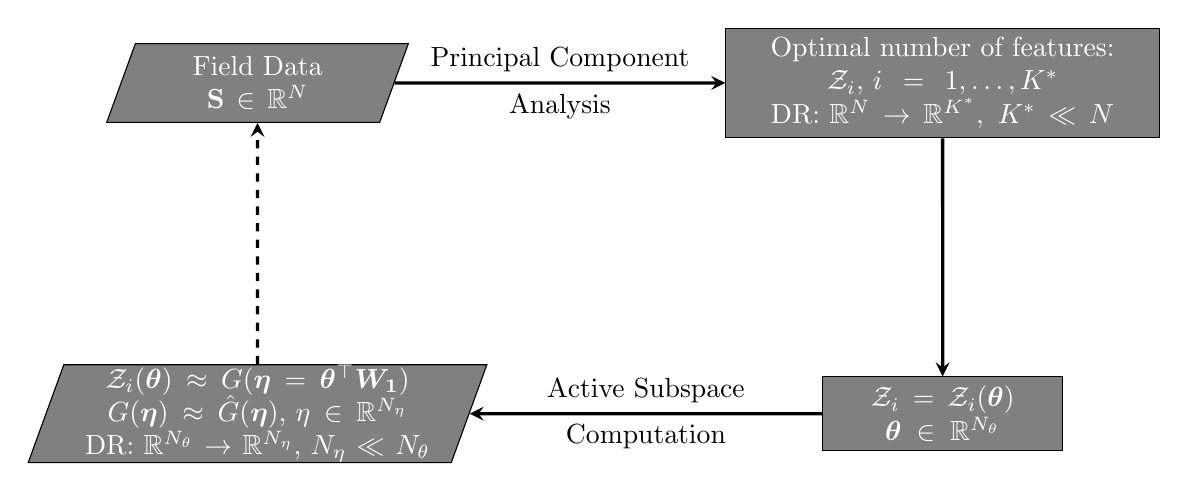
\begin{tikzpicture}[node distance=1.2cm,scale=0.6, every node/.style={scale=1.0}]

\node (field) [io, text width=6em] {Field Data\\ $\mat{S}\in\mathbb{R}^N$};

\node (pca) [process, right of=field, text width=15em, xshift=7.5cm] {Optimal number of features: \\ 
$\mathcal{Z}_i$, $i=1,\ldots,K^\ast$\\
DR: $\mathbb{R}^{N}\rightarrow \mathbb{R}^{K^\ast},~K^\ast\ll N$};

\draw [arrow] (field) -- node[above] {Principal Component} node [below] {Analysis} (pca);

\node (zk) [process, below of=pca, text width=8em, yshift=-3.0cm] {$\mathcal{Z}_i=\mathcal{Z}_i(\bm{\theta})$\\
$\bm{\theta}\in\mathbb{R}^{\Nt}$};

\draw [arrow] (pca) -- (zk);

\node (as) [io, below of=field, text width=14em, yshift=-3.0cm]{$\mathcal{Z}_i(\bm{\theta})\approx 
G(\bm{\eta}=\bm{\theta}^\top \bm{W_1})$\\ 
$G(\bm{\eta})\approx \hat{G}(\bm{\eta})$, $\eta\in\mathbb{R}^{N_\eta}$\\
DR: $\mathbb{R}^{\Nt}\rightarrow \mathbb{R}^{N_\eta}$, $N_\eta\ll \Nt$};

\draw [arrow] (zk) -- node [above] {Active Subspace} node [below] {Computation} (as);

\draw [arrow,dashed] (as) -- (field);

\end{tikzpicture}
\end{center}
\caption{Flow diagram illustrating the sequence of steps and associated dimension reduction (DR) in the PCAS method.}
\label{fig:fd}
\end{figure}
%
Once a surrogate for each feature is built, the field of interest can be reconstructed as shown in Figure~\ref{fig:re}.
%
%
\begin{figure}[htbp]
\begin{center}
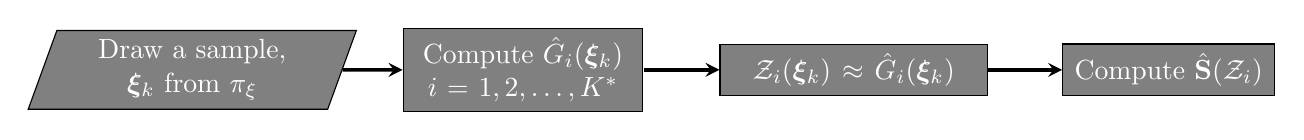
\begin{tikzpicture}[node distance=1.2cm,scale=0.6, every node/.style={scale=1.0}]

\node (s1) [io, text width=7.5em] {Draw a sample, $\bm{\xi}_k$ from $\pi_\xi$};

\node (s2) [process, right of=s1, text width=8em, xshift=3.0cm] {Compute $\hat{G}_i(\bm{\xi}_k)$\\ $i=1,2,\ldots,K^\ast$};

\draw [arrow] (s1) -- (s2);

\node (s3) [process, right of=s2, text width=9em, xshift=3.0cm] {$\mathcal{Z}_i(\bm{\xi}_k)\approx\hat{G}_i(\bm{\xi}_k)$};

\draw [arrow] (s2) -- (s3);

\node (s4) [process, right of=s3, text width=7em, xshift=2.8cm] {Compute $\hat{\mat{S}}(\mathcal{Z}_i)$};

\draw [arrow] (s3) -- (s4);

\end{tikzpicture}
\end{center}
\caption{Flow diagram illustrating the sequence of steps for reconstructing the field of interest.}
\label{fig:re}
\end{figure}











\bigskip
%%
\section{Electron Beam Melting: Multiphysics Model}
\label{sec:model}

Electron beam melting (EBM) is an additive manufacturing process of fusing powder particles, layer-upon-layer, 
using an electron beam as the energy source. The process is typically used in the case of metals and its alloys.
Multiple passes of  a low power electron beam is used for heating and sintering the powder bed prior to selective
melting. For the application problem in this study, we focus on the thermo-mechanical behavior of an AM part
produced by the EBM process. For this purpose, we have developed a finite element-based thermal analysis
model to simulate the thermal response of the part and a finite element-based mechanical model that uses
the part's thermal
response to estimate the residual stress in the part at the end of the cooling phase. Note that the stress is computed
at the end of a single pass of the electron beam. In this study, the two models are
weakly coupled i.e. the temperature history of the part is used as an input heat load for the mechanical model. 
Finite element analysis is performed using Abaqus~\cite{Hibbitt:2001}, a commercially available software. 

Our analysis is based on stress development in an AM part as a result of a single scan of an 
electron beam along its
length. A layer thickness, 50~$\mu$m and a part of dimensions (in mm), 2$\times 1.5\times 0.65$ is used as shown
in Figure~\ref{fig:PartwMesh}~(left). 
The process of laying the new powder on bulk material formed by previous scans is simulated 
by activating the initially deactivated elements representing the powder layer. To mitigate computational cost
associated with FEA, a non-uniform mesh is employed wherein a finer mesh is considered for the powder
region where the heat flux is applied. A gradually coarsening mesh is considered for the bulk material, significantly far 
from the heat source as shown in Figure~\ref{fig:PartwMesh}~(right). The mesh consists of 13,200 nodes and 
10,752 elements in total. 
%
\begin{figure}[htbp]
\begin{center}
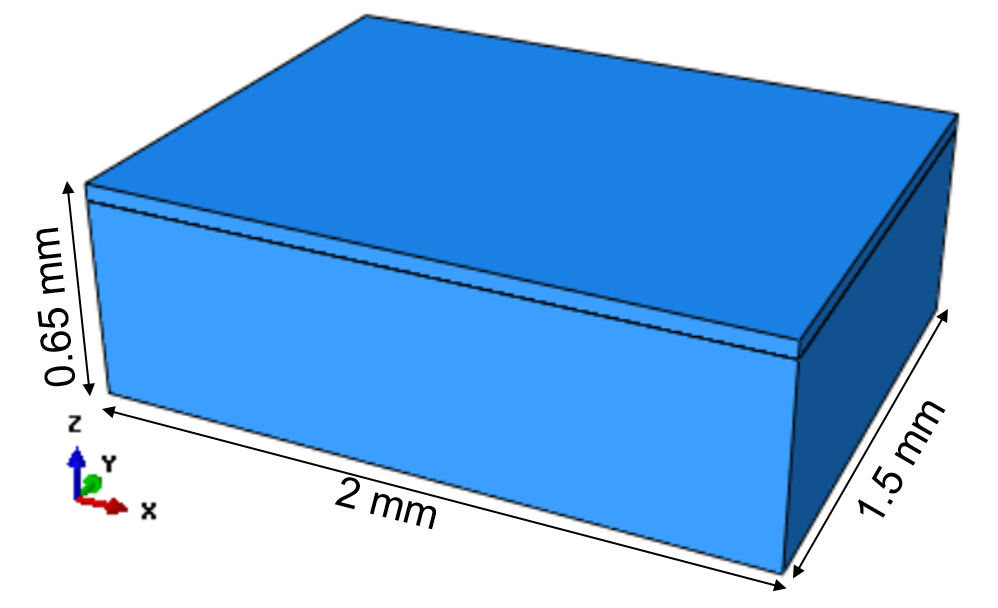
\includegraphics[width=0.4\textwidth]{./Figures/EBM_PartwXYZ} 
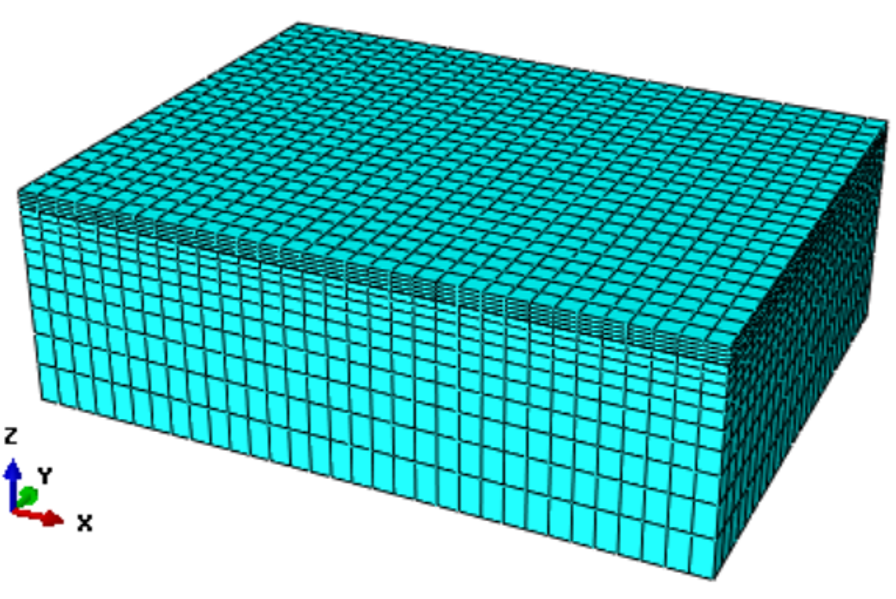
\includegraphics[width=0.4\textwidth]{./Figures/meshwXYZ}
\end{center}
\caption{Part geometry and the corresponding mesh as modeled in Abaqus}
\label{fig:PartwMesh}
\end{figure}
%
The material used to manufacture the part is considered to be Ti-6Al-4V and its
thermophysical properties considered in the finite element analysis are provided in Table~\ref{tab:matProp}.
%
\begin{table}[htbp]
\centering
\caption{Thermophysical properties of Ti-6Al-4V~\cite{Fu:2014}}
\label{tab:matProp}
\vspace{1mm}
\begin{tabular}{ ll }
\toprule
    Density (kg $/$m$^3$) & 4428\\
    Solidus Temperature ($^\circ$ C) & 1605 \\
    Liquidus Temperature ($^\circ$ C) & 1655\\
    Latent heat (J$/$kg) & 365000\\
    Elastic Modulus (GPa) & 110 \\
    Poisson's ratio & 0.41\\
    Yield strength (MPa) & 825\\
\bottomrule
\end{tabular}
\end{table}
%%%

\subsection{Thermal Model}
\label{sub:thermal}

The governing equation for the heat transfer analysis \cite{Zinoviev:2016} is given by:
\begin{equation}\label{eq_thermal}
\rho {C_p}\frac{{\partial T}}{{\partial t}} = -\nabla\cdot ({\kappa}\nabla T) + Q_e - Q_r 
\end{equation}
where $T$, $\rho$, $C_p$, $\kappa$, $Q_e$ denote the local temperature, average density, specific heat,  thermal 
conductivity, 
and the applied heat flux respectively. A single scan is considered along the x-direction at the top surface of the part. 
Heat flux due to the moving electron beam is modeled as a Gaussian~\cite{Vastola:2016} according to the following
equation:
%
\begin{equation}\label{eq_heatFlux}
Q_e = \frac{2P}{\pi r^2 d}\frac{1}{5}\Big[-3\Big(\frac{z}{d}\Big)^2-2\frac{z}{d}+5\Big]\exp\left({\frac{-2((x-vt)^2+y^2)}{r^2}}\right)
\end{equation}
%
where $P=\alpha IV$ denotes the power associated with the electron beam for a given absorptivity~($\alpha$),
current~(I), and voltage~(V). The quantities: $v$, $r$, and $d$ denote  the beam velocity or scan speed,
beam spot radius, and penetration depth respectively. The external heat flux is illustrated using temperature
contours on the top surface in Figure~\ref{fig:thermal}~(left) and along x-z plane passing through the center of the part in
Figure~\ref{fig:thermal}~(right). 
%
\begin{figure}[htbp]
\begin{center}
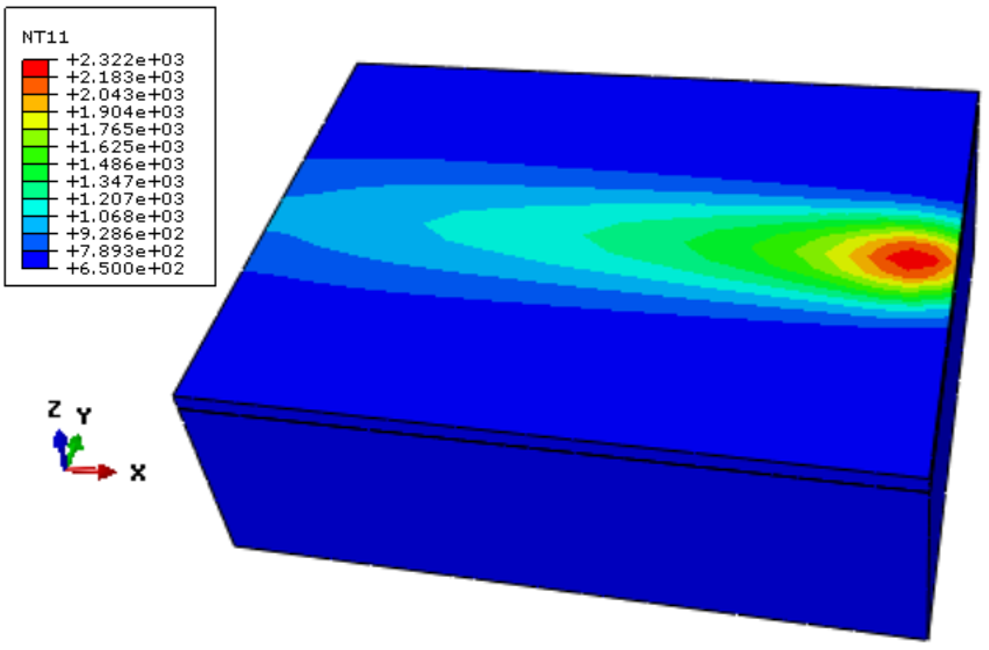
\includegraphics[width=0.42\textwidth]{./Figures/NT11Nom3D} 
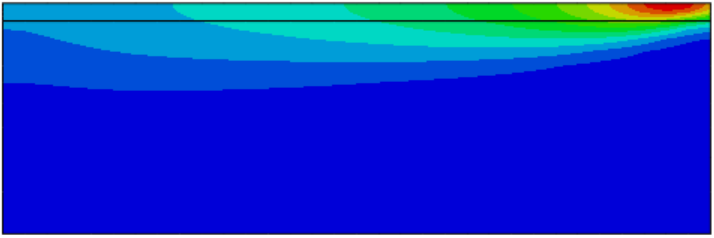
\includegraphics[width=0.42\textwidth]{./Figures/NT11Nom} 
\end{center}
\caption{Left: Temperature contours associated with the moving electron beam as a heat source. Right:
Temperature contours in the x-z plane passing through the center of the part once the electron beam is 
turned off.}
\label{fig:thermal}
\end{figure}
%

The laser beam radius~($r$) and the thermal penetration depth are fixed at 200 and 28
microns respectively. The powder is pre-heated to a temperature, $T_0$ prior to the scan using fixed temperature
boundary conditions at the lateral sides as well as the bottom of the part. Heat transfer in the part occurs by two
mechanisms: First, by means of thermal conduction due to temperature gradients especially along the depth (x-z plane),
and second, by means of radiative losses from the exposed surface of the part denoted as $Q_r$ in~\eqref{eq_thermal}.
The radiative heat flux, $Q_r$ is modeled using the Stefan-Boltzmann law i.e., 
$Q_r=\sigma_\text{SB}\epsilon(T^4-T_a^4)$, where
$\sigma_\text{SB}$, $\epsilon$, and $T_a$ denote the Stefan-Boltzmann constant, emissivity of the top surface, and the ambient
temperature respectively. Note that convective losses are not considered since the manufacturing process is 
assumed to be
carried out in vacuum. As discussed later in Section~\ref{sec:results}, the beam power~($P$), scan speed~($v$), and 
pre-heat temperature of the powder bed~($\theta_0$) are considered as process control parameters~($\bm{\theta_p}$)
in our analysis using the surrogate model. The temperature history of the part determined using the thermal model
is used as an input to the mechanical model (one way coupling) to compute residual stress in the AM part as 
discussed in the following section. 

\subsection{Mechanical Model}
\label{sub:mech}

The governing equation for structural analysis \cite{Megahed:2016} is given by:
%
\begin{equation}\label{eq_mechanical}
\nabla \cdot \mat{\sigma}+f = 0
\end{equation}
%
where $\sigma$ and $f$ denote the stress tensor and the internal forces respectively. From Hooke's law, the stress
tensor ($\mat{\sigma}$) is proportional to the total strain~($\epsilon^T$). Material stiffness tensor, $\mat{C}$ is the
proportionality constant. The constitutive relationship is given as follows:
%
\be
\mat{\sigma} = \mat{C}\epsilon^e
\ee
%
where $\mat{C}$ is the fourth-order material stiffness tensor and $\epsilon^e$ denotes
the elastic strain. The total strain 
$\epsilon^T$ can be decomposed as follows:
%
\be
\epsilon^T = \epsilon^e + \epsilon^p+ \epsilon^t
\ee
%
where $\epsilon^p$, and $\epsilon^t$ denote
plastic and thermal strains respectively~\cite{Megahed:2016}. 
The plastic strain is modeled by considering elastic 
perfectly-plastic~\cite{Zhao:2015} condition in the model. Thermal strain is calculated  from the thermal expansion 
constitutive relationship: $\varepsilon^t = \alpha_{t}\Delta T$, where $\alpha_t $ is the thermal expansion coefficient.
The boundary surfaces in the X-direction and Y-direction are constrained in the x-
coordinates and y-coordinates respectively. The bottom surface is considered fixed in all coordinates.
The temperature history at each node, obtained using the thermal model in~\ref{sub:thermal}, is used to
compute the strain tensor, $\sigma$. Hence, the mechanical response is dependent on the thermal response
of the part but not vice versa. The coupling between the two models is therefore regarded as \textit{one-way}
or \textit{weak}~\cite{Debroy:2017} (A \textit{strong} or \textit{two-way} coupling assumption is computationally
unaffordable, since it requires multiple back-and-forth iterations between the two models for convergence, at 
each time step). 
The von Mises stress at the end of the cooling process
is considered as the residual stress in the AM part~\cite{Vastola:2016}. 
It is considered as the quantity of interest~(QoI) in our analysis for 
demonstrating the methodology proposed earlier in Section~\ref{sec:method}. The stress contours are illustrated
in Figure~\ref{fig:subSmises} 
%
\begin{figure}[htbp]
\begin{center}
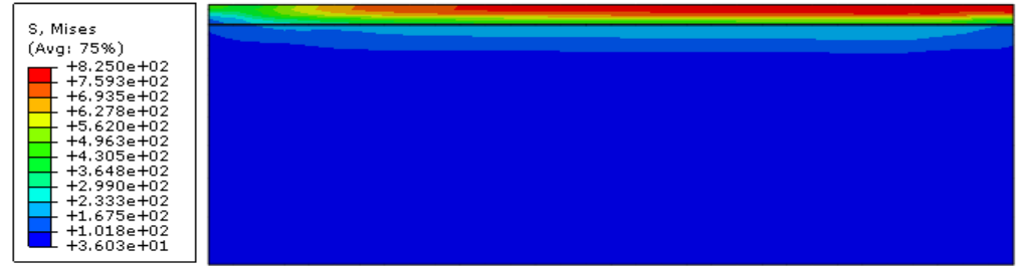
\includegraphics[width=0.6\textwidth]{./Figures/SMisesNom} 
\end{center}
\caption{von Mises stress contours in the x-z plane passing through the center of the part after it has cooled
down to the ambient temperature.}
\label{fig:subSmises}
\end{figure}
%
The contour plot in Figure~\ref{fig:subSmises} clearly indicates that the residual stress in the part attains higher
values near the top surface and diminishes quickly along the depth of the part. It can thus be said that thermal
strain due to the applied heat flux is the dominant contributor to the residual stress in the present set-up. 

Simulations are performed on a workstation with a system configuration: Intel~Core~i7-4790~CPU, 
3.60 GHz with 16GB RAM. It is observed that on average the thermal model takes 20 minutes, and the
mechanical model takes 10 minutes to complete the simulation pertaining to a single pass of the
electron beam. Note, however, that the simulation duration depends on the choice of
values for the set of inputs. Moreover, a weak coupling assumption leads to a computational time of 30
minutes to generate 1 training point for the surrogate model. On the other hand, a strong coupling assumption 
would lead to 150 minutes considering 5 iterations are needed for convergence to generate 1 training point. 


























\bigskip
%
\section{Results}
\label{sec:results}

In this section, we provide relevant details pertaining to the construction of the surrogate model to predict
the field of interest, i.e. the
residual stress in the AM part cross-section using the PCAS method in~\ref{sub:surr}. The surrogate is used to map
the process control parameters and the material properties to the residual stress field. The computational efficiency
enabled by the surrogate is exploited to perform a global sensitivity analysis of the inputs in~\ref{sub:gsa}. Finally, the
surrogate is used for reliability prediction for the AM part by estimating the probability of failure based on residual stress
in~\ref{sub:reliability}.

\subsection{Surrogate Model}
\label{sub:surr}

A surrogate model is constructed for the residual stress field at the cross-section of the part 
(x-z plane in Figure~\ref{fig:PartwMesh}) passing through its center. We will refer to this plane
as x$^c$-z$^c$ in the remainder of this paper. The surrogate maps three sets of
parameters, namely, the process control parameters~($\bm{\theta_P}$), mechanical properties~($\bm{\theta_M}$),
and thermal properties~($\bm{\theta_T}$) to the stress field. The set of process control parameters includes
the beam power~($P$), scan speed~($v$), and the pre-heat temperature~($T_0$). Mechanical properties
include the yield strength~($Y$), the elastic modulus~($E$), and the bulk density~($\rho$). Thermal 
properties include specific heat~($C_p$) and bulk thermal conductivity~($\kappa$). Note that $C_p$ and $\kappa$
are considered to be functions of the local temperature, $T$. Specifically, a polynomial of degree 2 was fit
to a set of data pertaining to the variation of $C_p$ and $\kappa$ with temperature (20~K--1655~K), 
provided in~\cite{Fu:2014} as shown in Figure~\ref{fig:Cp_kappa}.
%
\begin{figure}[htbp]
\begin{center}
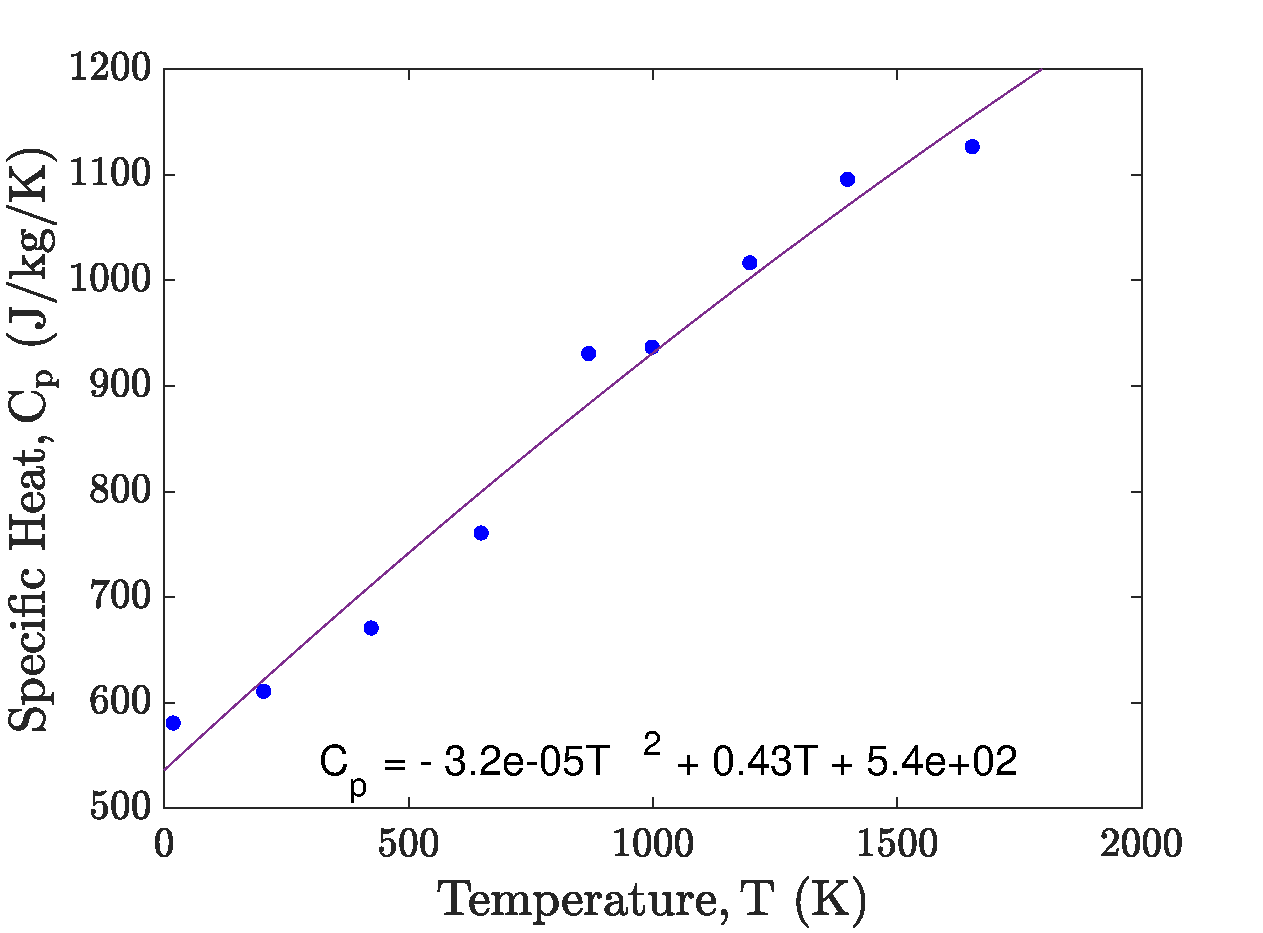
\includegraphics[width=0.42\textwidth]{./Figures/cp_fit}
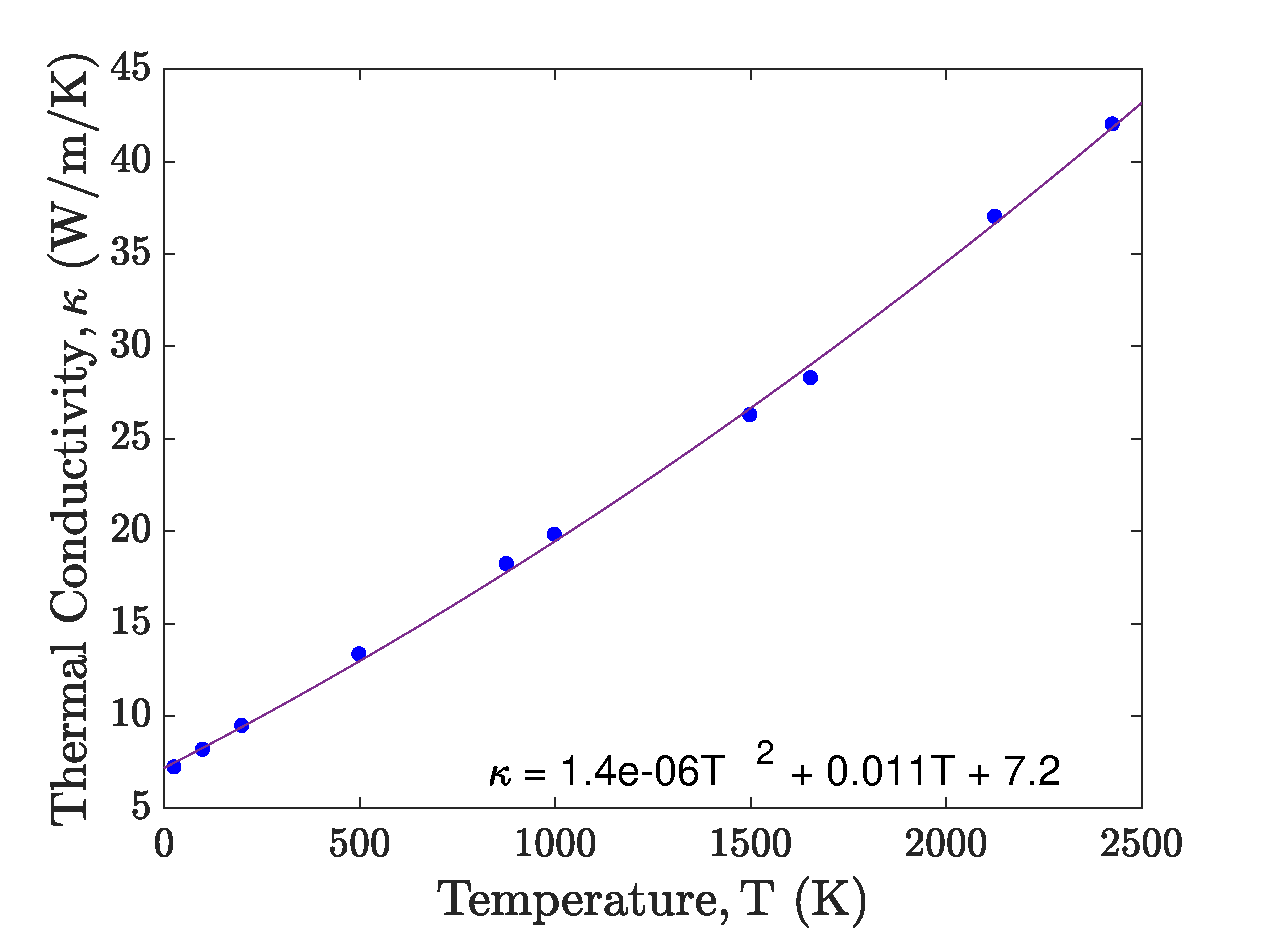
\includegraphics[width=0.42\textwidth]{./Figures/kappa_fit}
\end{center}
\caption{A second degree polynomial fit to specific heat~($C_p$), and thermal conductivity~($\kappa$) data
for a temperature range, [20,1655](K). Note that the data provided in~\cite{Fu:2014} was used to determine
the coefficients of the regression fit.}
\label{fig:Cp_kappa}
\end{figure}
%
Hence, a total of 12 parameters~($\bm{\theta}$) are mapped to the stress field including coefficients of the polynomial fits
corresponding to $C_p$ and $\kappa$. A uniform prior: $[0.9\bm{\theta}^\ast, 1.1\bm{\theta}^\ast]$, 
where $\bm{\theta}^\ast$ denotes a vector of nominal values,
is considered for each parameter. Nominal values of the mechanical properties: $Y$, $E$, and $\rho$ are provided
in Table~\ref{tab:matProp}. Nominal values of the process control parameters and temperature coefficients for
the thermal properties are provided in Table~\ref{tab:remain}.
%
\begin{table}[htbp]
\centering
\caption{EBM process control parameters and temperature coefficients for $C_p$~($C_i$'s) and $\kappa$~($D_i$'s).}
\label{tab:remain}
\vspace{1mm}
\begin{tabular}{ ll }
\toprule
Scan Speed, $v$~(mm/s) & 500 \\
Beam Power, $P$~(W) & 160 \\
Pre-heat Temperature, $T_0$~(C) & 650 \\
Specific heat, $C_p$ = $C_0+C_1T+C_2T^2$~(J/kg/K) & 540~($C_0$),0.43~($C_1$),$-3.2\times 10^{-5}$~($C_2$) \\
Thermal Conductivity, $\kappa$ = $D_0+D_1T+D_2T^2$~(W/m/K) & 7.2~($D_0$),0.011~($D_1$),$1.4\times 10^{-6}$~($D_2$) \\
\bottomrule
\end{tabular}
\end{table}
%%%

Residual stress is initially computed at the x$^c$-z$^c$ plane for 10 pseudorandom samples in the 12-dimensional
input domain. Stress data is simulated on a 2-dimensional non-uniform grid comprising 32 points along the
length~(x$^c$) and 14 points along the height~(z$^c$) as highlighted in Figure~\ref{fig:RS_comp}~(left).
As mentioned earlier in Section~\ref{sec:model}, a 
finer mesh is used near the part surface since sharp thermal gradients lead to a larger amount of stress
in this region as shown in Figures~\ref{fig:subSmises} and~\ref{fig:RS_comp}.  Following the flow diagram
in Figure~\ref{fig:fd}, the first step involves a principal component analysis on the field data. 
Algorithm~\ref{alg:pca}) is used for this purpose. However, the reconstructed field failed
the verification and the validation tests in this case, i.e. $\varepsilon_0^{\text{ver}}$ and $\varepsilon_0^{\text{val}}$
were greater than 0.1. A new set of 5 model realizations were added at subsequent iterations and the iterative
procedure was observed to converge in 2 iterations. Error estimates for each iteration are provided in
Table~\ref{tab:error}.
%
\begin{table}[htbp]
\centering
\caption{Convergence of the surrogate model as a function of iterations and sample size.}
\label{tab:error}
\vspace{1mm}
\begin{tabular}{ ccll}
\toprule
Iteration &  Sample Size & $\varepsilon_i^{\text{ver}}$ & $\varepsilon_i^{\text{val}}$\\
0 & 10 & 0.06 & 0.31 \\
1 & 15 & 0.09 & 0.28 \\
2 & 20 & 0.04 & 0.07\\
\bottomrule
\end{tabular}
\end{table}


In Figure~\ref{fig:pca}, we plot the reconstruction error, $\varepsilon_\mathcal{R}^\infty$ against the number of
principal components, $K$. 
%
\begin{figure}[htbp]
\begin{center}
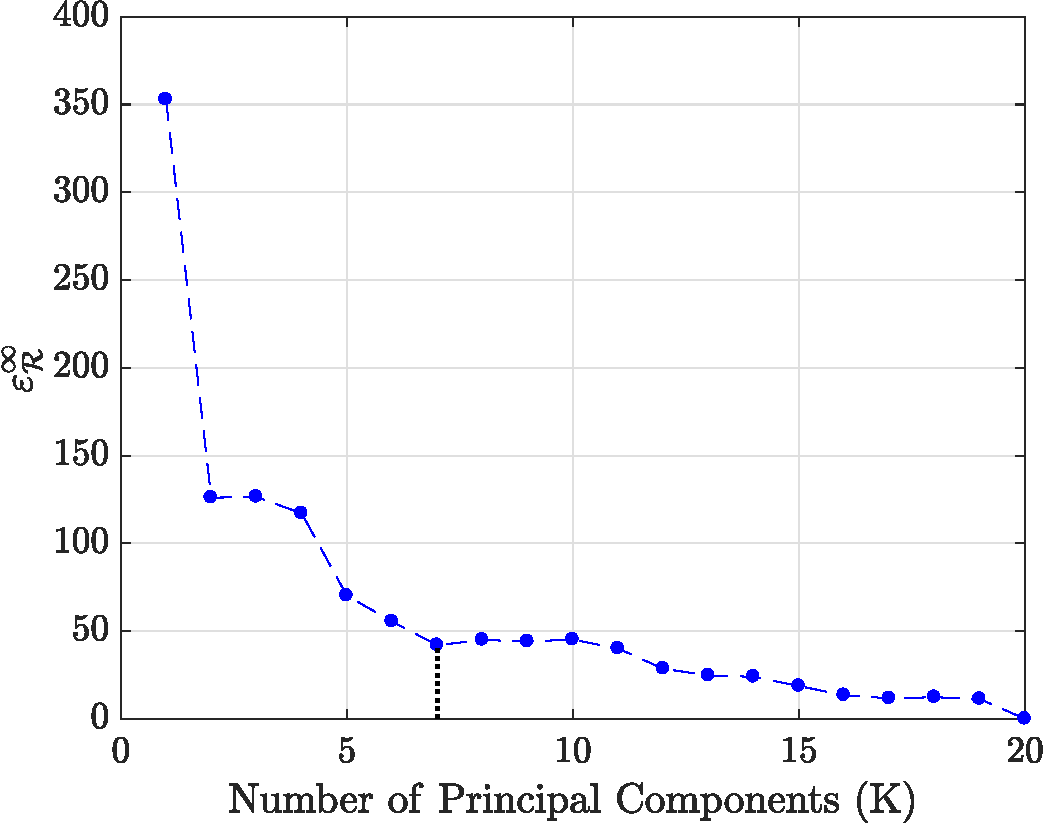
\includegraphics[width=0.42\textwidth]{./Figures/error_PCA}
\end{center}
\caption{A plot of the reconstruction error, $\varepsilon_\mathcal{R}^\infty$ as a function of the
number of principal components obtained using the iterative PCA approach in Algorithm~\ref{alg:pca}.}
\label{fig:pca}
\end{figure}
%
As expected, $\varepsilon_\mathcal{R}^\infty$ is observed to mostly decrease with the number of components. 
A monotonic behavior is not expected since the components only capture partial information in the data. It 
appears that most of the information is captured using 20 components since the error is almost 0. However,
building the surrogate for 20 features would potentially entail a large computational effort depending upon the
application. Here, we consider that $K^\ast$ = 7 components are optimal since the error plateaus as the number of
components increase from 7 to 10 indicating diminishing returns. Thus, the residual stress field is reconstructed
using a surrogate for each of these $K^\ast$ components~($\mathcal{Z}_i$'s, $i = 1,2,\ldots,K^\ast$).
The dimensionality of the output space is therefore reduced 
from $\mathbb{R}^{14\times 32=448}\rightarrow \mathbb{R}^7$. We now shift our focus on dimension reduction
in the input space.

As discussed earlier in~\ref{sub:as}, each feature can be expressed as a function of $\bm{\theta}$ in the physical
space. Note that $\bm{\theta}:\{\bm{\theta_P}\cup\bm{\theta_M}\cup\bm{\theta_T}\}$. An active subspace computation
was performed using a regression-based approach~\cite{Constantine:2015, Vohra:2019}
for estimating the gradient and the available set of 20 realizations for each $\mathcal{Z}_i$. 
The eigenvalue spectrum of the matrix, $\hat{\mathbb{C}_i}$ for each $\mathcal{Z}_i$ is shown in Figure~\ref{fig:as}.
The variability of a given $\mathcal{Z}_i$ in terms of the active variables, $\bm{\eta}$ regarded as the sufficient summary
plot~(SSP) is also included in each case.
%
\begin{figure}[htbp]
\begin{center}
\begin{subfigure}{0.35\textwidth}
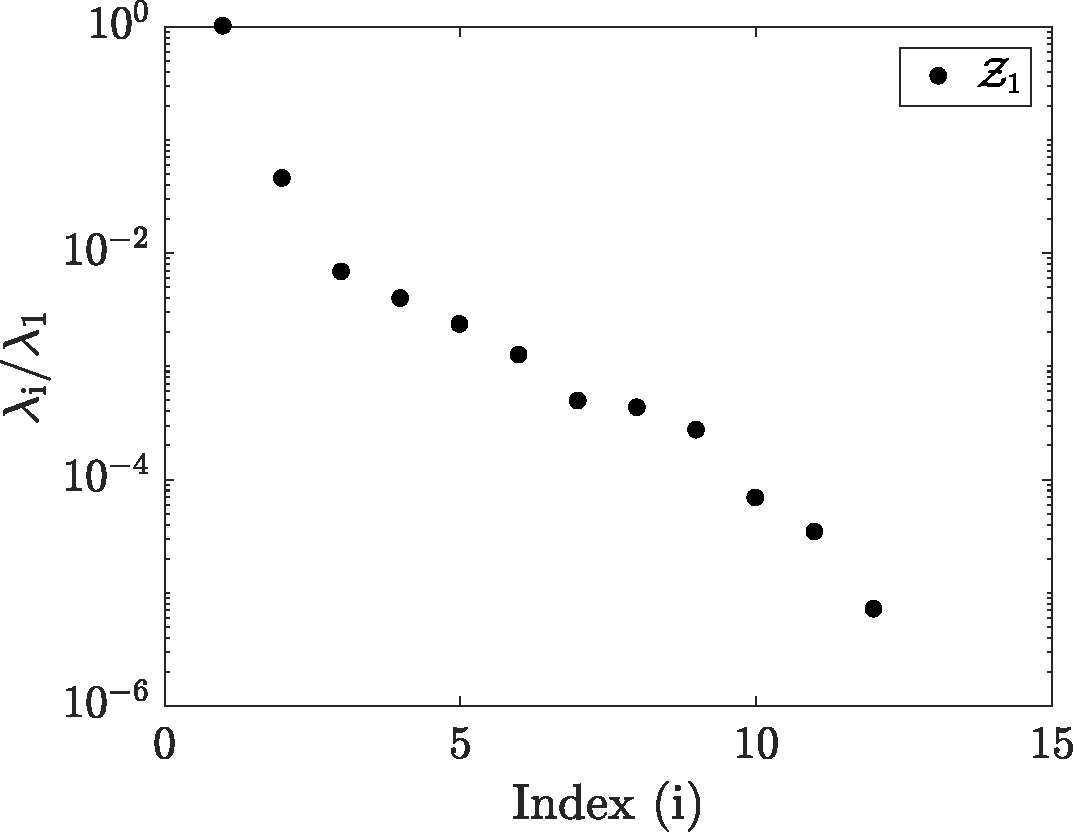
\includegraphics[width=0.65\textwidth]{./Figures/eig_Zf1} 
\\
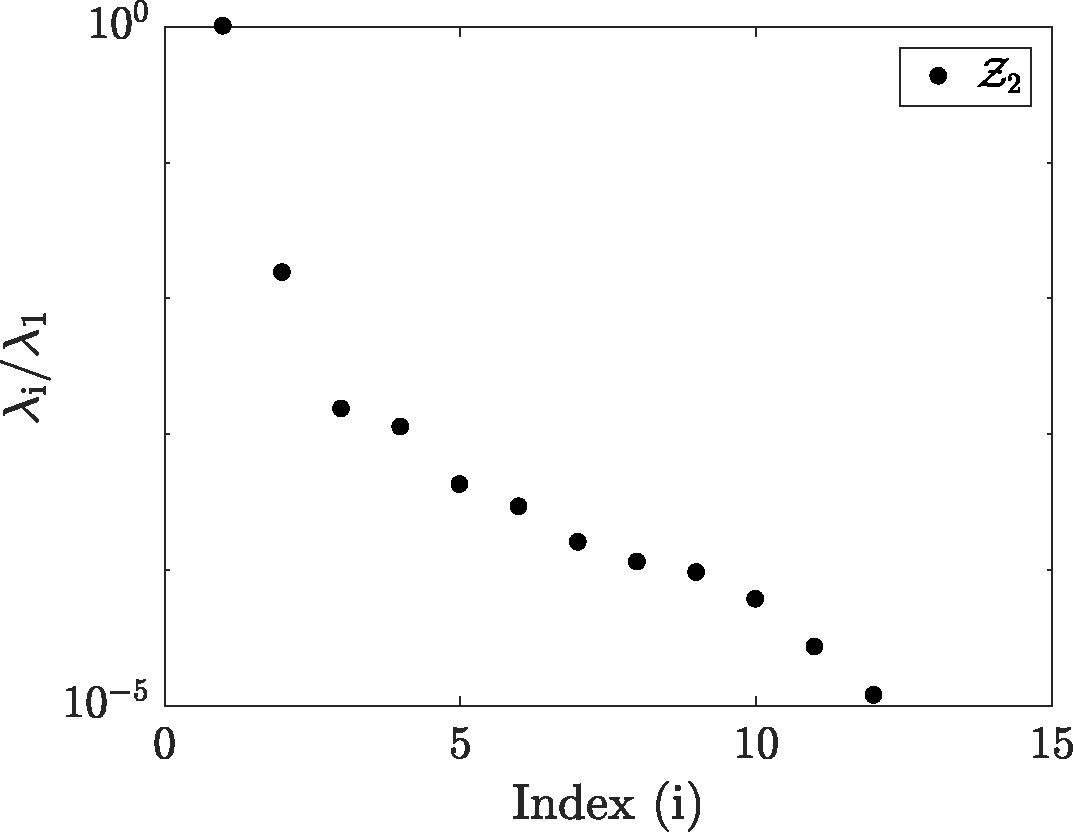
\includegraphics[width=0.65\textwidth]{./Figures/eig_Zf2} 
\\
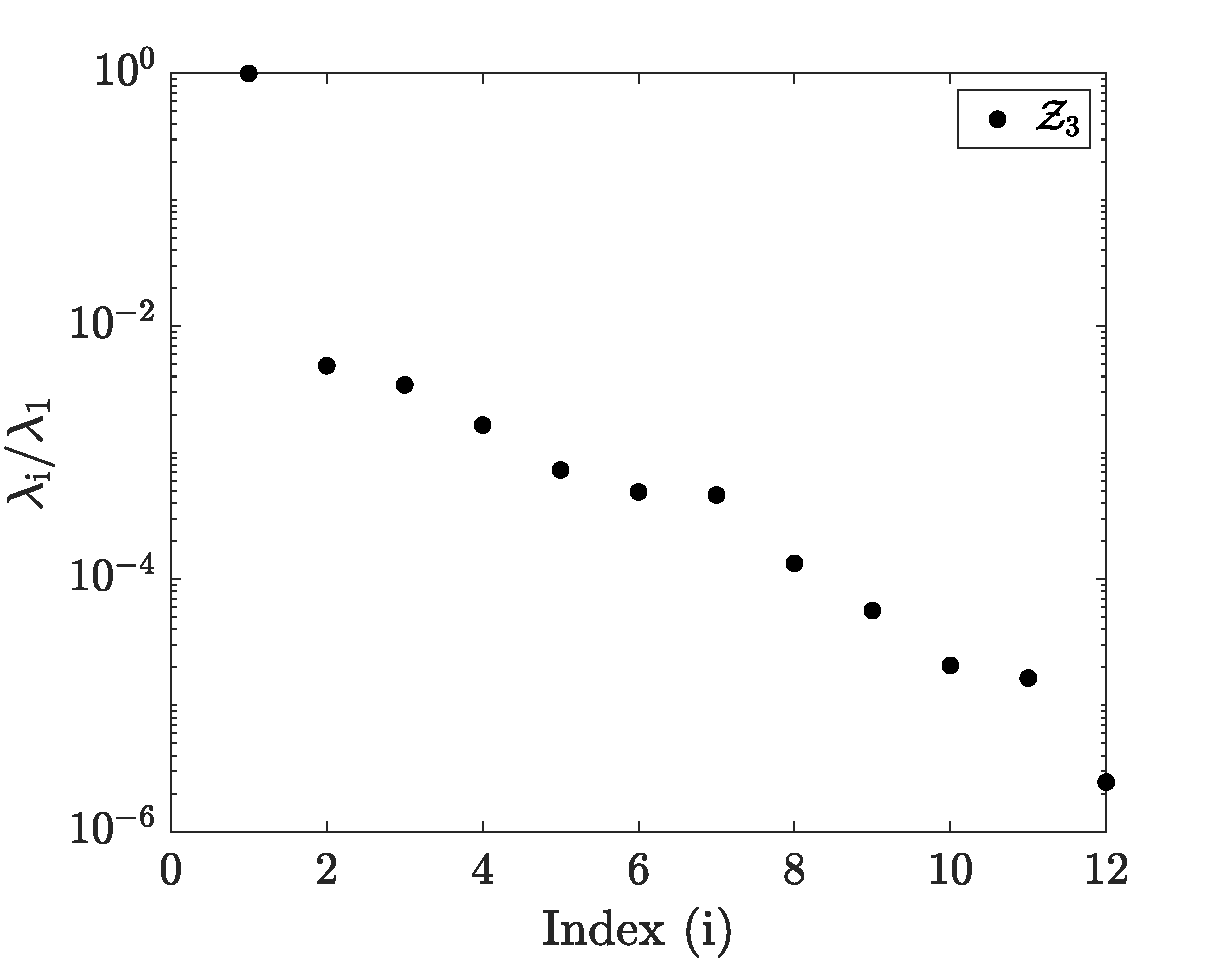
\includegraphics[width=0.65\textwidth]{./Figures/eig_Zf3} 
\\
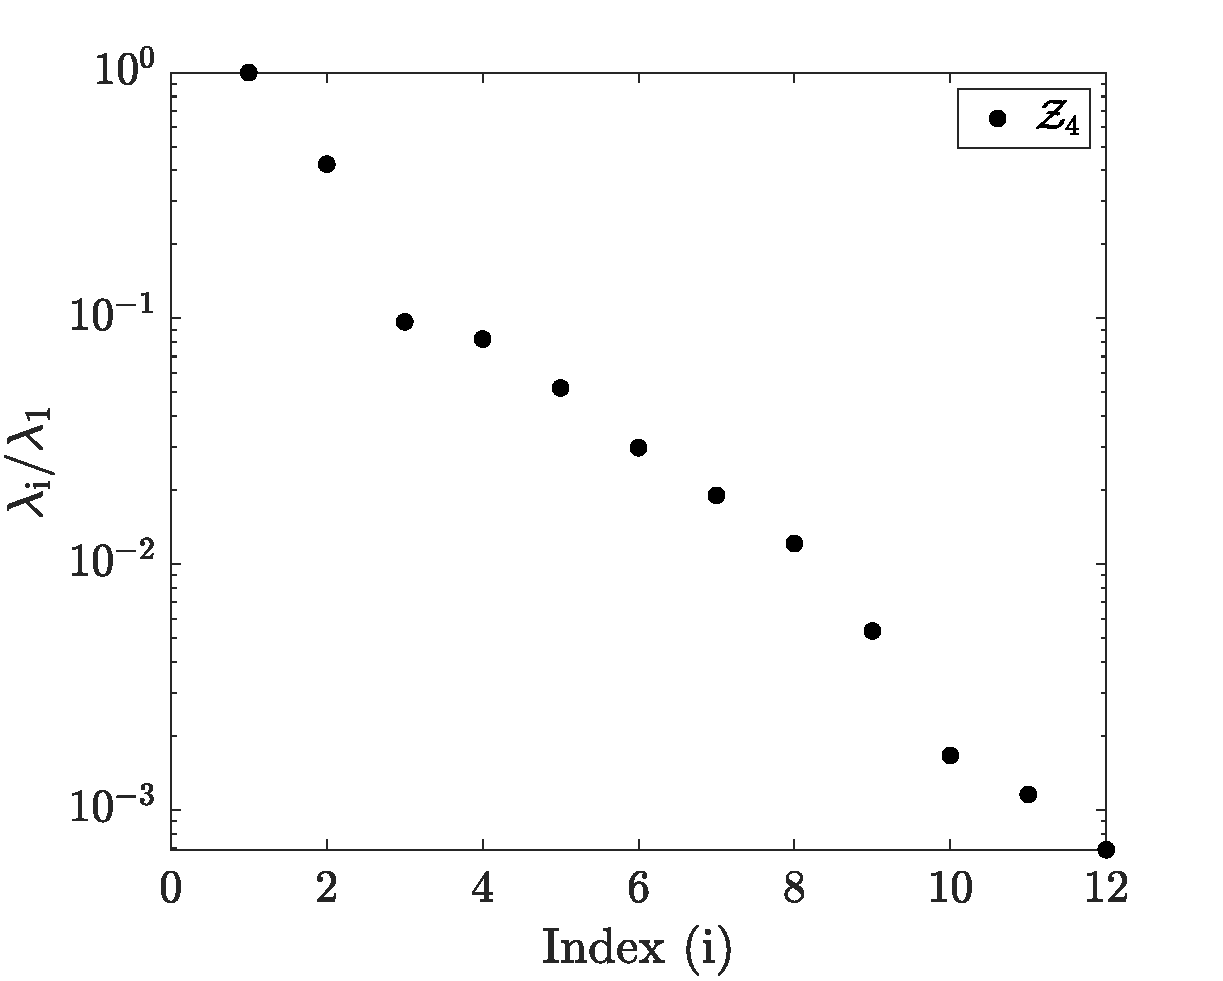
\includegraphics[width=0.65\textwidth]{./Figures/eig_Zf4} 
\\
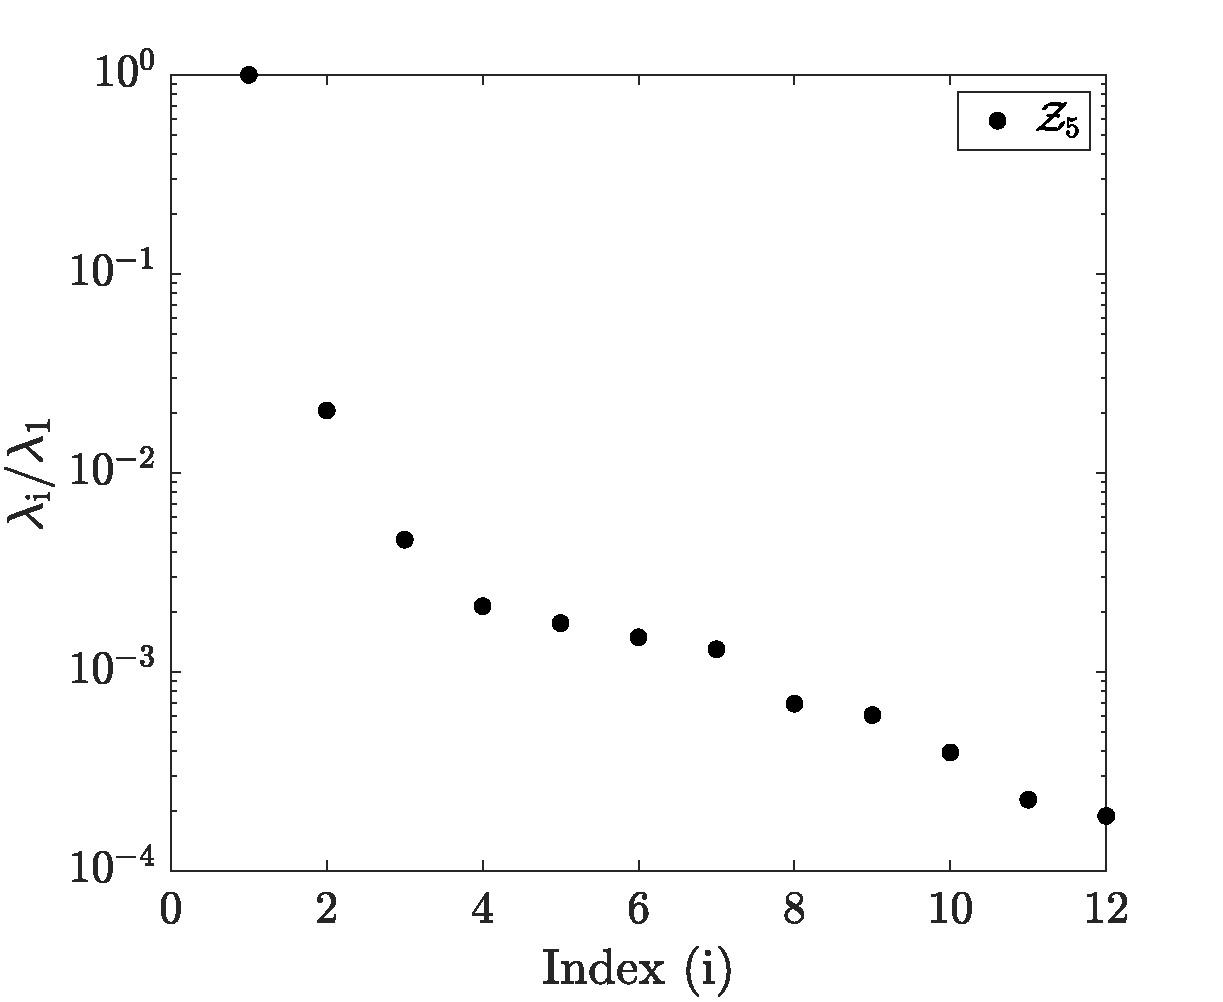
\includegraphics[width=0.65\textwidth]{./Figures/eig_Zf5} 
\\
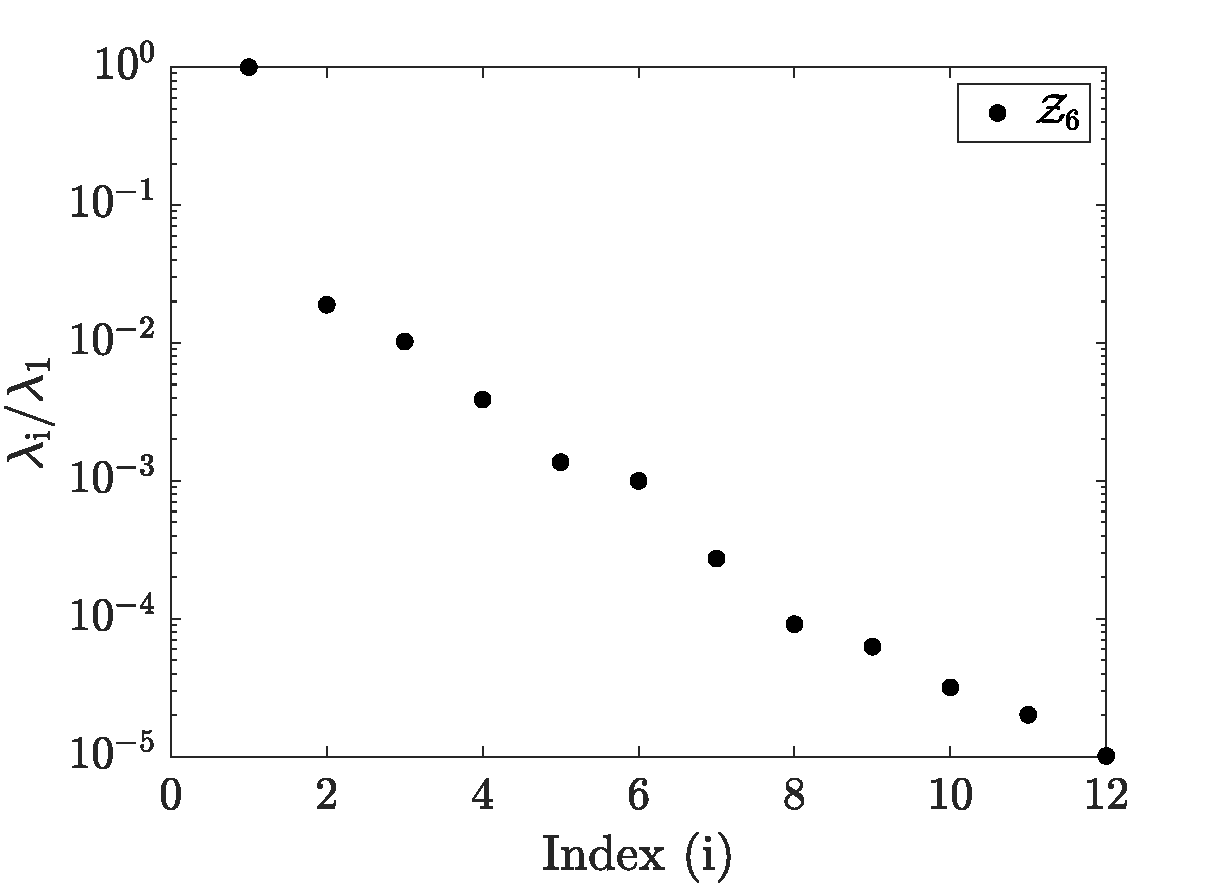
\includegraphics[width=0.65\textwidth]{./Figures/eig_Zf6} 
\\
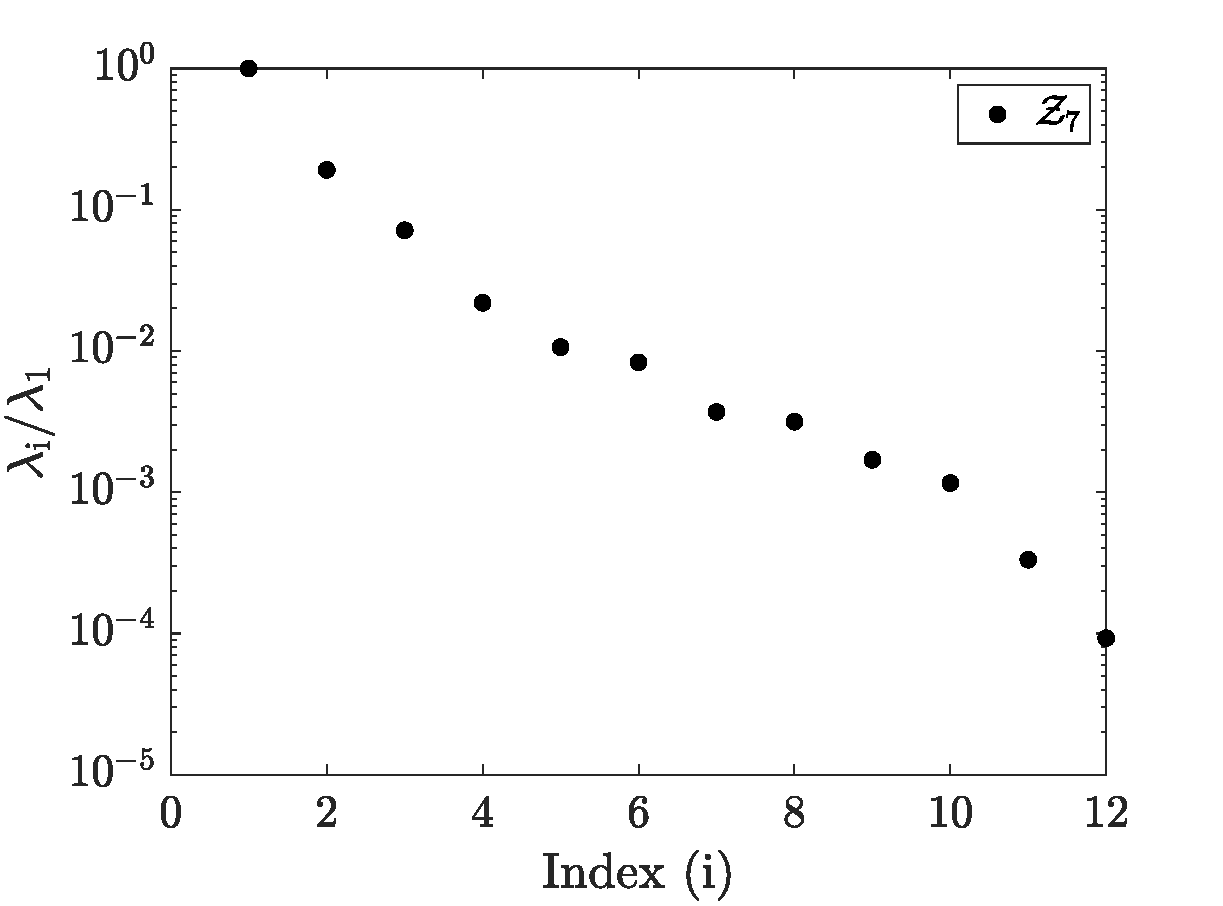
\includegraphics[width=0.65\textwidth]{./Figures/eig_Zf7} 
\end{subfigure}
\hspace{-0.5cm}
\begin{subfigure}{0.35\textwidth}
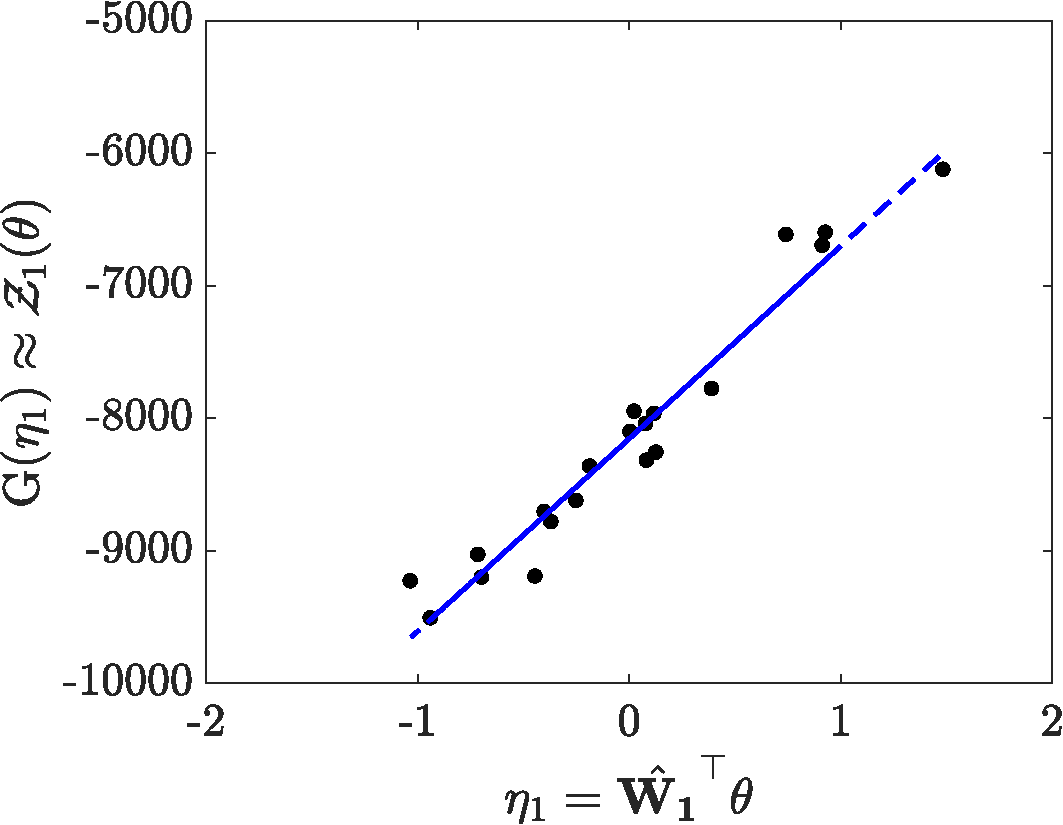
\includegraphics[width=0.65\textwidth]{./Figures/SSP_Zf1} 
\\
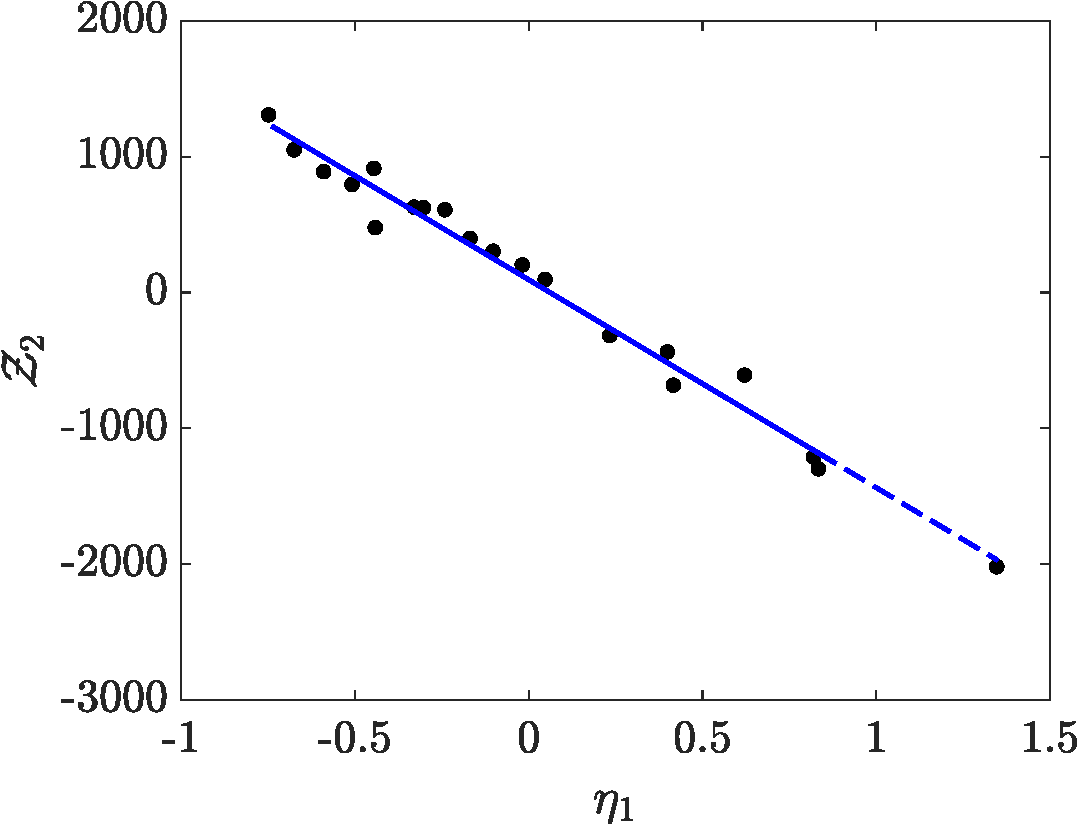
\includegraphics[width=0.65\textwidth]{./Figures/SSP_Zf2} 
\\
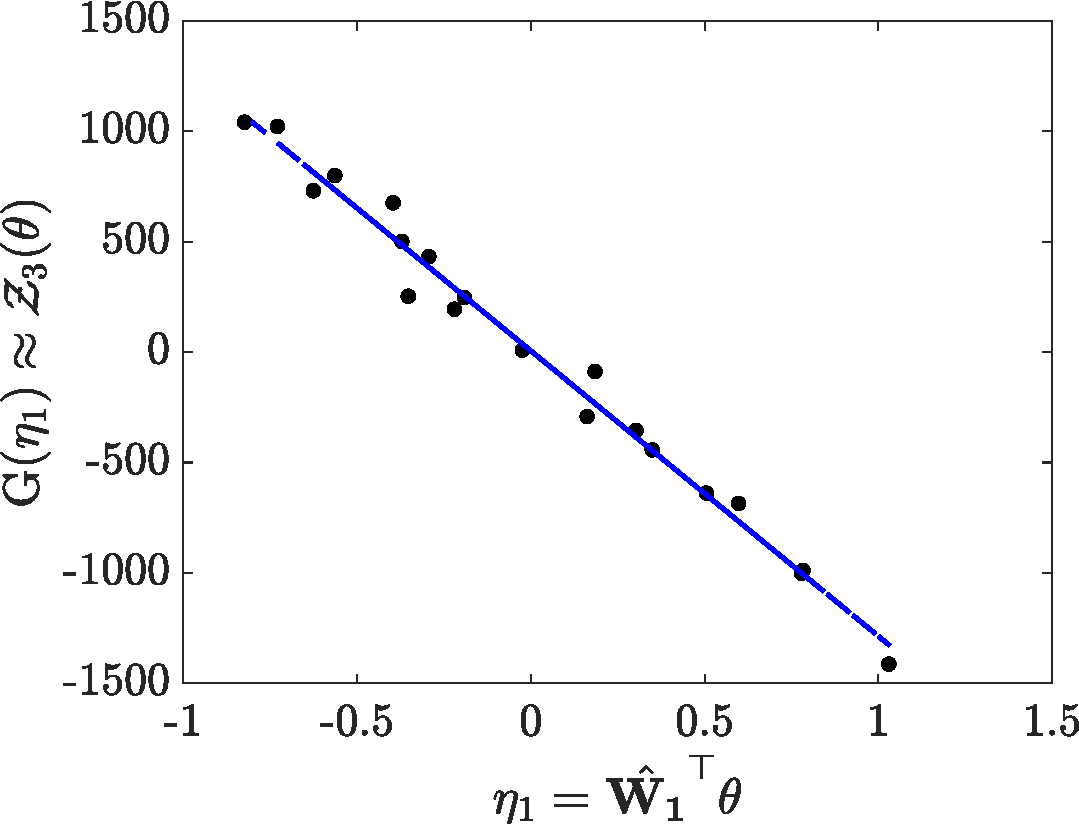
\includegraphics[width=0.65\textwidth]{./Figures/SSP_Zf3} 
\\
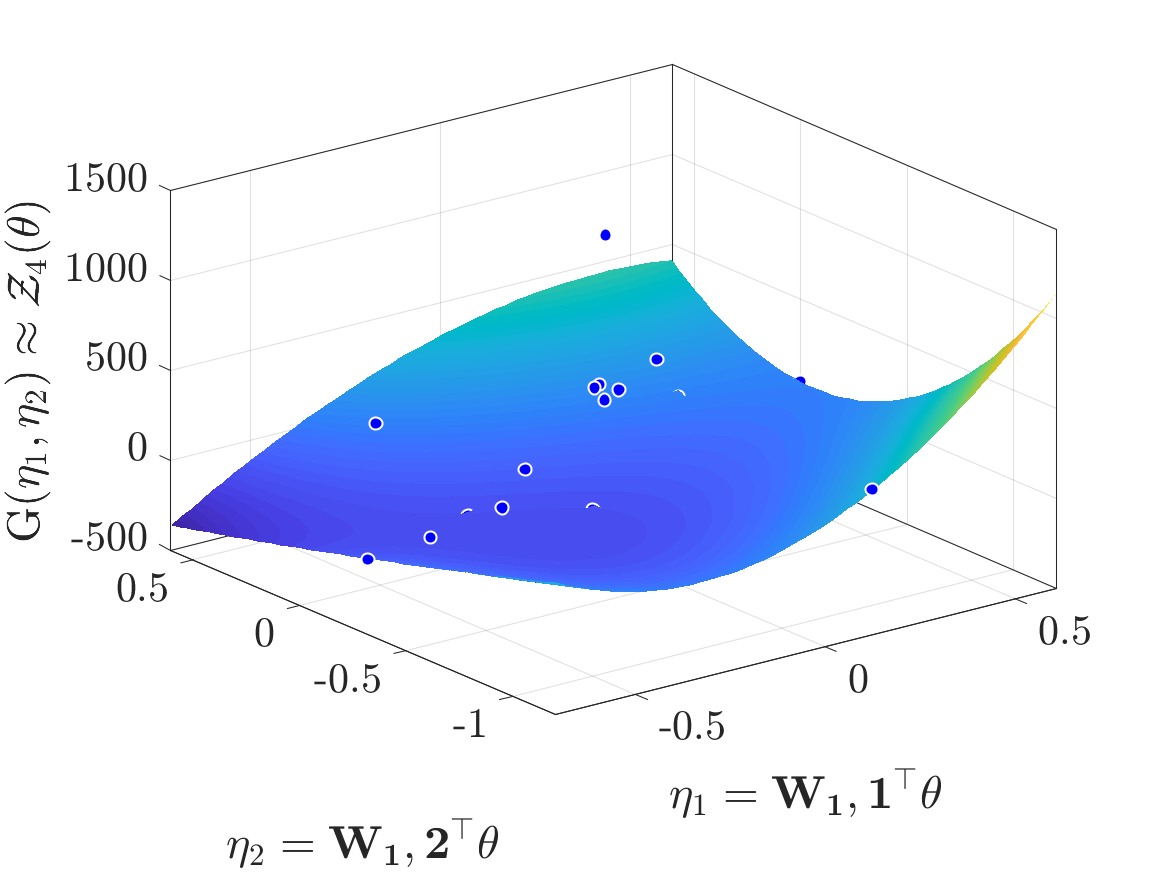
\includegraphics[width=0.65\textwidth]{./Figures/SSP2D_Zf4} 
\\
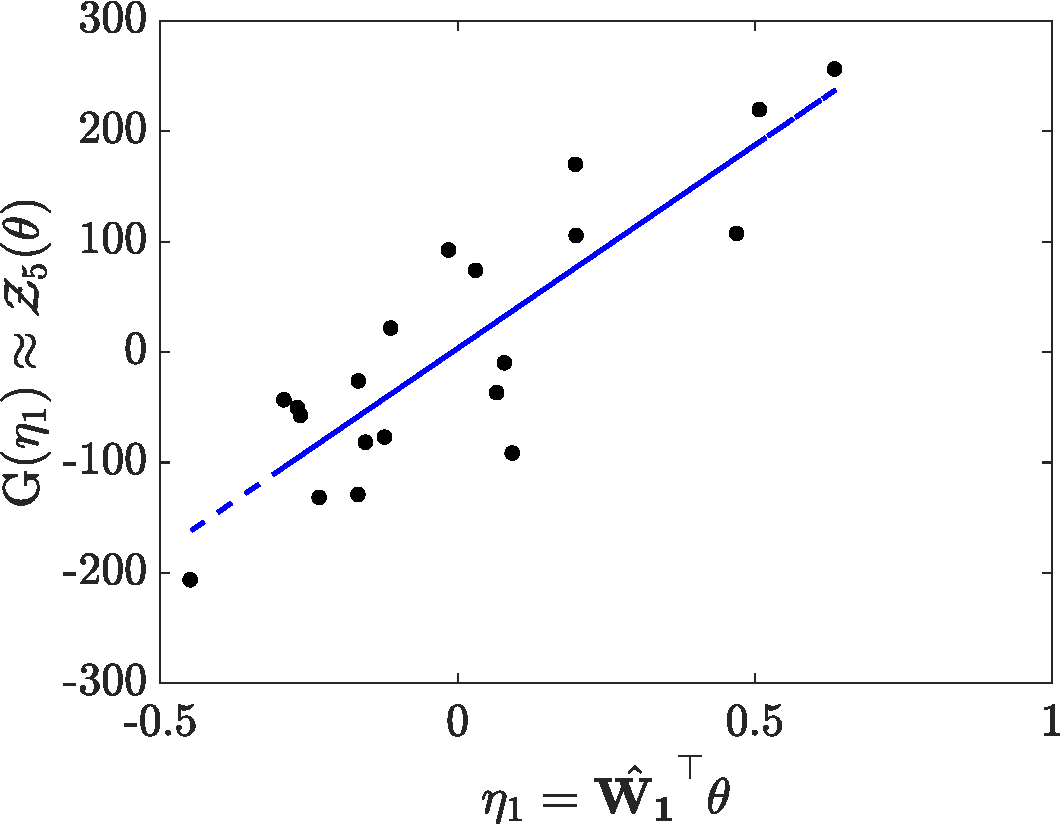
\includegraphics[width=0.65\textwidth]{./Figures/SSP_Zf5} 
\\
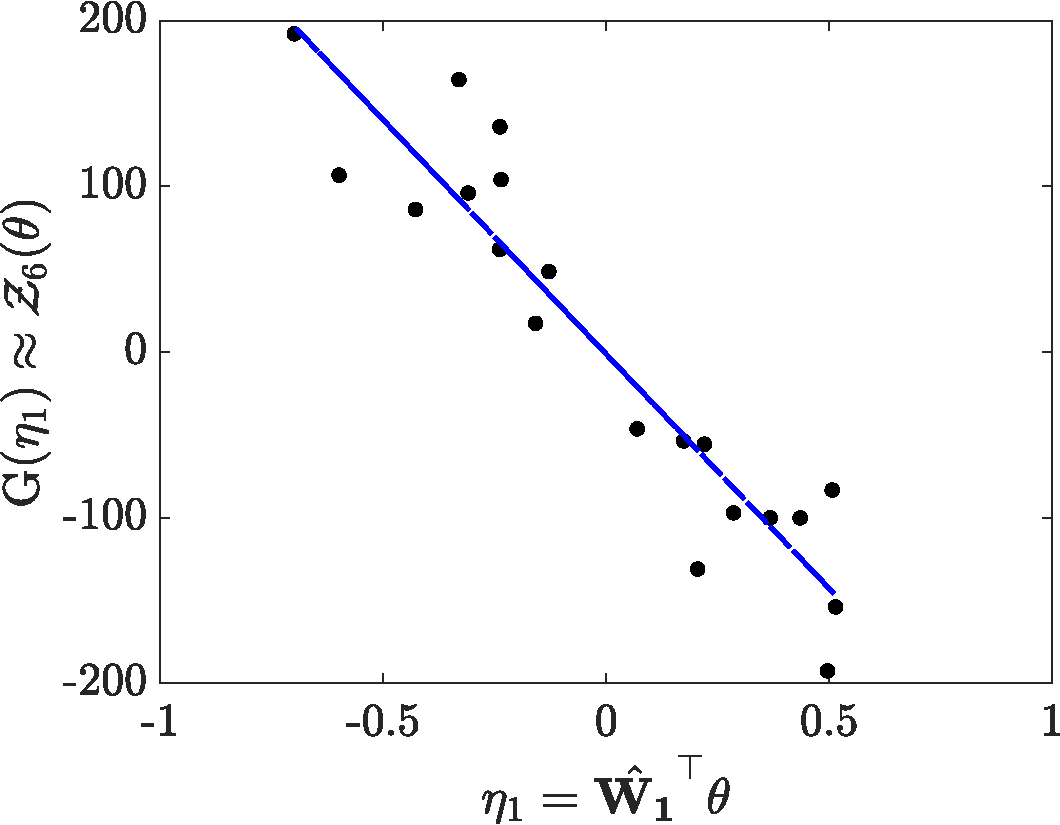
\includegraphics[width=0.65\textwidth]{./Figures/SSP_Zf6} 
\\
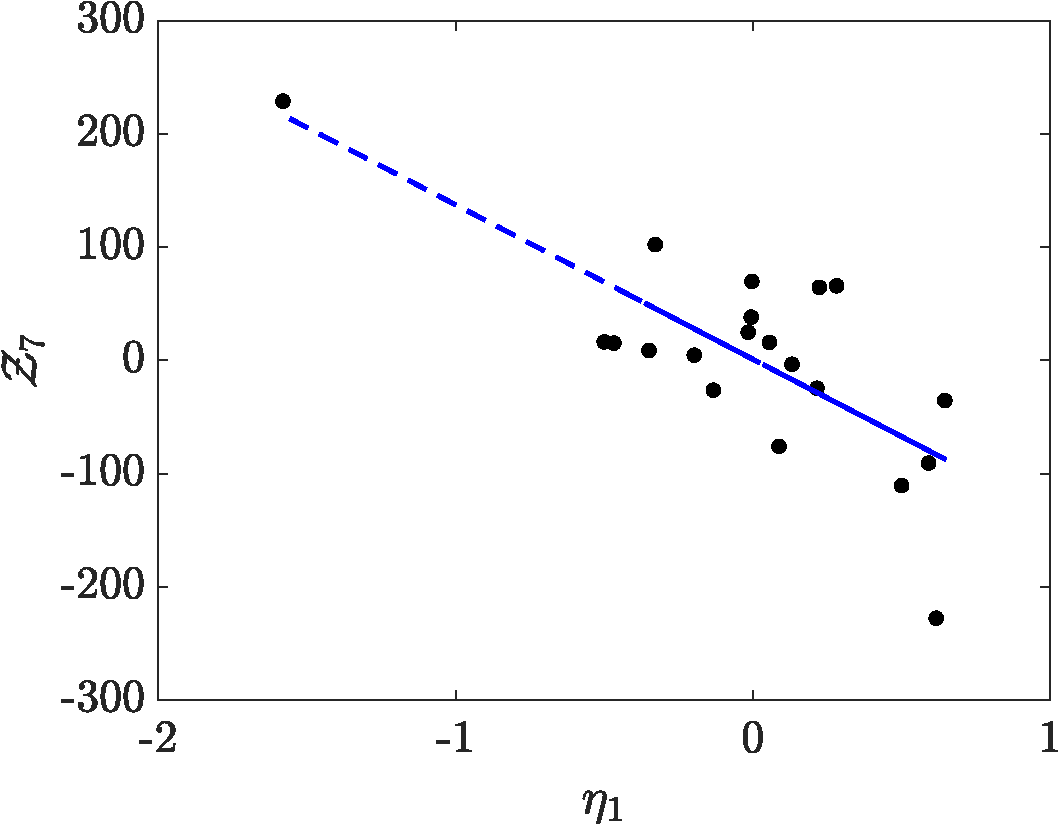
\includegraphics[width=0.65\textwidth]{./Figures/SSP_Zf7} 
\end{subfigure}
\end{center}
\caption{Eigenvalue spectrum and the corresponding SSP for each $\mathcal{Z}_i$.}
\label{fig:as}
\end{figure}
%
From these plots, it is observed that in all cases except $\mathcal{Z}_4$, a 1-dimensional active
subspace captures the variability in the feature with reasonable accuracy. More specifically, the
eigenvalue spectrum exhibits a significant jump between the first and second eigenvalue. Consistent
with these observations, a straight-line fit to the realizations of the feature in the SSP is observed to be
reasonably accurate. In the case of $\mathcal{Z}_4$, $\lambda_1$ and $\lambda_2$ are comparable, and
a significant jump exists between $\lambda_2$ and $\lambda_3$. Therefore, a 2-dimensional active
subspace is considered in this case as shown. Polynomials of degrees 3 and 2 along $\eta_1$ and
$\eta_2$ respectively were used to construct the regression surface. The regression-fits in each case
serves as a surrogate for the corresponding feature, $\mathcal{Z}_i$. Therefore, a sample $\bm{\xi}_i$
corresponding to $\bm{\theta}_i$ in the physical space is propagated through each surrogate to estimate
$\mathcal{Z}_i$'s and hence, the residual stress field as shown using a flow diagram in Figure~\ref{fig:re}.
The individual surrogates for $\mathcal{Z}_i$'s thus constitute the overall surrogate model that maps the 
physical variables to the stress field. We will refer to this overall surrogate model as the \textit{composite
surrogate} in the remainder of this paper. 

Dimension reduction in the input space is therefore found to be from $\mathbb{R}^7\rightarrow\mathbb{R}^2$.
Therefore, using the proposed PCAS method, significant dimension reduction in both input and output
spaces is accomplished leading enormous gains in computational efficiency for the considered application.

\subsubsection{Surrogate Verification and Validation}
\label{subsub:vnv}

As mentioned earlier in this section, 20 model realizations were needed to obtain a surrogate model with
reasonable accuracy with respect to the reconstructed residual stress field in the x$^c$-z$^c$ plane. 
Specifically, the verification and validation errors were found to be approximately 0.04 and 
0.07 respectively. In other words, the stress field reconstructed using the
composite surrogate model achieves an accuracy of about 7$\%$ on average. Although these error estimates
are based on a relatively small sample size, they seem reasonable considering that the validation test samples
were generated using Latin hypercube sampling (LHS) that explores the entire input domain more uniformly
as compared to Monte Carlo sampling. Therefore, the PCAS approach appears to provide a reasonably 
accurate surrogate coupled with enormous computational gains which makes the analyses pertaining to
the present application affordable. 

Figure~\ref{fig:RS_comp} illustrates a side-by-side comparison of stress distribution in the $x^c$-z$^c$ plane,
computed using the FEM~(left) with those generated using the composite surrogate~(right) using the same
set of input conditions. The two plots
are observed to be in close agreement with each other.  
%
\begin{figure}[htbp]
\begin{center}
\begin{subfigure}{0.15\textwidth}
\vspace{10mm}
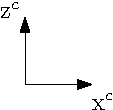
\includegraphics[width=0.5\textwidth]{./Figures/xczc} 
\end{subfigure}
\hspace{-1.5cm}
\begin{subfigure}{0.35\textwidth}
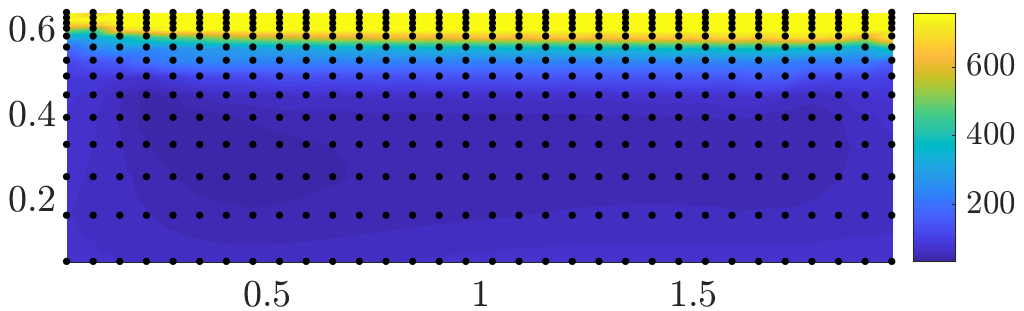
\includegraphics[width=1.0\textwidth]{./Figures/origZ_sam13} 
\end{subfigure}
\hspace{0.25cm}
\begin{subfigure}{0.35\textwidth}
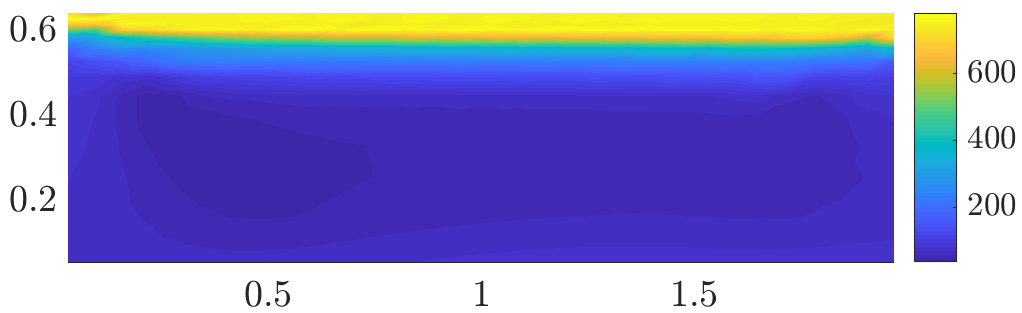
\includegraphics[width=1.0\textwidth]{./Figures/recZ_sam13} 
\end{subfigure}
\end{center}
\caption{Left: Residual stress field in the $x^c$-z$^c$ plane as generated using the Abaqus model with inputs, 
$\bm{\theta}_p$. The grid points in the 2D mesh used for finite element simulations are also highlighted. 
Right: Reconstructed stress field using the surrogate model using the same set of parameters. }

%: $v=535.23$~mm/s, $P$=148.27~W,
%$T_0$=641.03~K, $Y$=777.74~MPa, $E$=99.16~GPa, $\rho$=4187.25~kg/m$^3$, $C_0$=546.43, $C_1$=0.47,
%$C_2$~=~-~3.07$\times$10$^{-5}$, $D_0$=6.84, $D_1$=0.01, $D_2$=1.47$\times$10$^{-6}$.}
\label{fig:RS_comp}
\end{figure}

\subsubsection{Hotspot Identification}
\label{subsub:hotspot}

As mentioned earlier in Section~\ref{sec:intro}, a large amount of residual stress severely impacts part
performance due to sub-optimal mechanical properties, reduced fatigue life, and geometrical inaccuracy. 
Identification of `stress hotspots' could thus be conceived as an important step in the manufacturing process.
Owing to the transient nature of the process conditions, material microstructure, and part configuration,
it would not be practicable to use the FEM. The surrogate model constructed using the PCAS method
proposed in this work could instead be used for the purpose.

For the present analysis, we focus on the hotspots in the $x^c$-z$^c$ plane, and any point in the 2D mesh
where the residual stress exceeds a threshold is considered as the hotspot. Figure~\ref{fig:hs} illustrates the 
location of the hotspots and associated stress values in the $x^c$-z$^c$ plane, for a particular set of
input conditions. A threshold value of 640~MPa is used. 
%
\begin{figure}[htbp]
\begin{center}
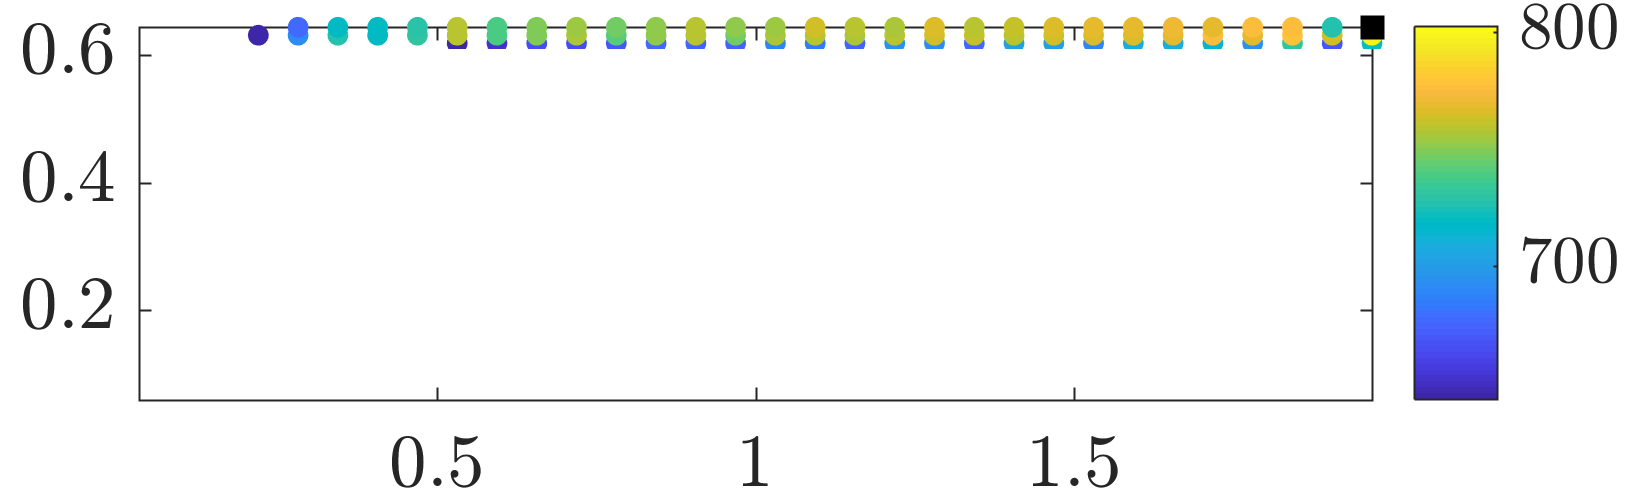
\includegraphics[width=0.42\textwidth]{./Figures/loc_hotspot10}
\end{center}
\caption{Location of the hotspots in the AM part and corresponding estimates of the von Mises stress
are indicated by means of a colorbar. The location of the peak stress is also shown using a black square.}
\label{fig:hs}
\end{figure}
%
As expected, the hotspots are located near the top surface of the part that experiences sharp temperature
gradients. For the purpose of identifying a global hotspot, the residual stress
field in the $x^c$-z$^c$ plane is simulated for 10$^6$ pseudorandom samples, generating using LHS
in the 12-dimensional input domain. Thus, stress distribution is obtained at each point in the mesh. 
The specific grid point with the maximum mean stress is regarded as the \textit{global hotspot},
denoted as P. Our findings reveal that P is in fact located at the top right corner of the $x^c$-z$^c$
plane, consistent with the location of the square in Figure~\ref{fig:hs}.
Figure~\ref{fig:kde_S} shows the PDF of stress distribution at point P. 
%
\begin{figure}[htbp]
\begin{center}
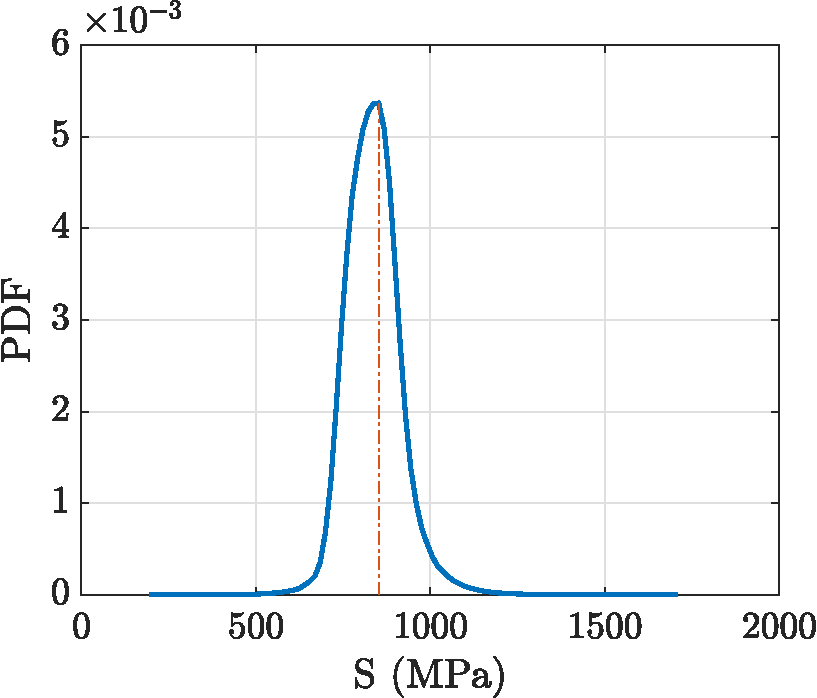
\includegraphics[width=0.42\textwidth]{./Figures/kde_S_mumax}
\end{center}
\caption{Probability density function~(PDF) of von Mises stress at P, generated using kernel density estimation in 
Matlab. The distribution is based on 10$^6$ evaluations and the mode value is estimated as 852.31~MPa.}
\label{fig:kde_S}
\end{figure}

\subsection{Global Sensitivity Analysis}
\label{sub:gsa}

The composite surrogate is further used for the purpose of global sensitivity analysis~(GSA). %
GSA is performed with respect to the stress value at point $P$, identified as the global hotspot
for residual stress in the $x^c$-z$^c$ plane as discussed earlier in~\ref{subsub:hotspot}. 

As mentioned earlier, the set of inputs in the physical space, $\bm{\theta}$ is classified into three
categories: process control parameters~($\bm{\theta_P}$), mechanical properties~($\bm{\theta_M}$), and
thermal properties~($\bm{\theta_T}$) of the alloy~(Ti6Al4V) used to manufacture the AM part. We focused
our efforts on determining the relative importance of $\bm{\theta_P}$, $\bm{\theta_M}$, and $\bm{\theta_T}$
wherein the individual parameters in each category are grouped together. Additionally, we investigate
relative importance of the process
control parameters and the material properties, i.e. $\bm{\theta_M}$ and $\bm{\theta_T}$ grouped together.
Such analyses with grouped variables would help focus the manufacturer's attention on the key
contributors to the variability in residual stress. For instance, depending upon the sensitivity estimates, the
manufacturer could focus on optimizing either the mechanical properties, thermal properties, or
the process control variables for minimizing the uncertainty in residual stress prediction. 
More importantly, optimizing the key contributors to the variability in residual stress would help maximize the reliability
of the finished product. 
 GSA was performed by estimating the main-effect and the total-effect Sobol' sensitivity
indices at 10$^5$ samples in the input domain using an algorithm based on 
Monte Carlo sampling~(MCS)~\cite{Sobol:2001}. The composite
surrogate was used to make the computations tractable. The estimated sensitivities for the two cases
are plotted in Figure~\ref{fig:gsa}.
%
\begin{figure}[htbp]
\begin{center}
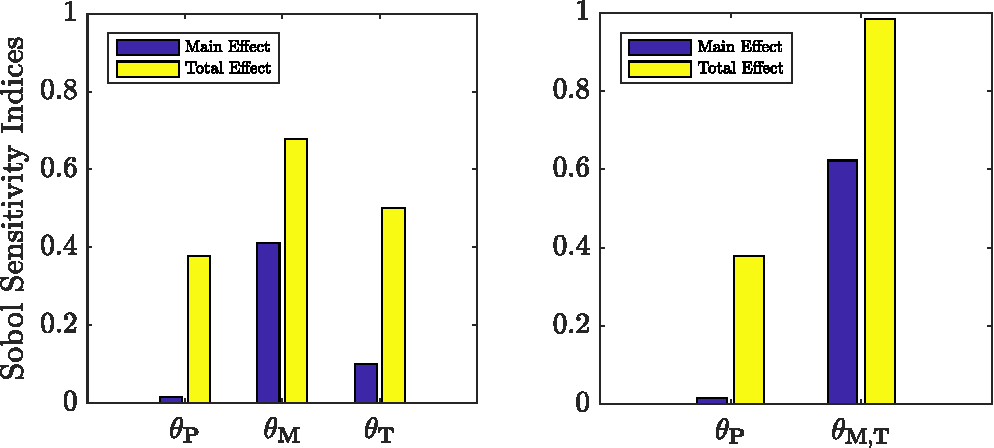
\includegraphics[width=0.65\textwidth]{./Figures/grouped_GSA}
\end{center}
\caption{Left: Sobol' sensitivity indices for the set of inputs grouped as process variables~($\bm{\theta_P}:v,P,T_0$), 
mechanical properties~($\bm{\theta_M}:Y,E,\rho$), and thermal properties~($\bm{\theta_T}:C_p,\kappa$).
Right: Sobol' sensitivity indices for the set of inputs grouped as process variables~($\bm{\theta_P}$), and material 
properties~($\bm{\theta_{M,T}}$).}
\label{fig:gsa}
\end{figure}
%
Several inferences can be made: The residual stress at P is most sensitive to the mechanical properties, followed 
by thermal properties of the alloy. Sensitivity towards the process control parameters is found to be relatively small. 
However, it must be noted that the interactions between $\bm{\theta_P}$, $\bm{\theta_M}$, and $\bm{\theta_T}$
are significantly large. Hence, the total-effect index of $\bm{\theta_P}$ indicates that the sensitivity towards the 
process variables is substantial. Therefore, optimizing the process parameters for minimizing residual
stress in the AM part could help improve its performance characteristics. 
Note that these results are dependent on the choice of nominal values as well as considered intervals
for the uncertain inputs. 

\subsection{Reliability Prediction}
\label{sub:reliability}

Reliability prediction involves estimating the probability of failure~($p_f$) of the AM part
corresponding to a defined failure criterion. Here, we estimate~$p_f$ based on the residual 
stress estimate at any location in
the part exceeding a given threshold. In other words, we aim to ensure that the residual stress
in the part does not exceed an upper bound and therefore, the performance characteristics of
the AM part are not severely degraded. Once again, we exploit the composite surrogate to
numerically estimate~$p_f$ as follows:
%
\be
\hat{p}_f = \frac{1}{N}\sum\limits_{k=1}^{N} \mathbb{H}\left[S^\ast-\max(\hat{\mat{S}})\right],
\ee
\label{eq:pf}
%
where $\hat{p}_f$ is the approximation to $p_f$, $N$ denotes the number of samples, $S^\ast$
denotes the limiting stress value, and $\max(\hat{\mat{S}})$ denotes the peak stress in the
x$^c$-z$^c$ plane based on the surrogate prediction. $\mathbb{H}[]$
is a Heaviside unit step function that assumes a value 1 for a positive argument and 0 for
a negative argument.
To ensure that $\hat{p}_f$ is a resonable approximation, it is estimated
using 10$^6$ samples in the input domain. Based on surrogate predictions at the generated set of samples,
the probability of failure using $S^\ast$~=~900~MPa is estimated to be 0.177. 


















































 

\bigskip
%
\section{Summary and Discussion}
\label{sec:conc}

In this paper, we have proposed an efficient approach, namely the PCAS method for constructing a surrogate model that 
maps a high-dimensional input to a high-dimensional output. The high-dimensional output is considered as a field quantity,
estimated at discrete points on a mesh used for numerical simulations. Computational efficiency is
accomplished by means of dimension reduction in the output space as well as the input space.
We begin by determining the optimal number of
components required to reasonably approximate the field using an iterative PCA approach~(Algorithm~\ref{alg:pca}).
The optimal set of components or important directions are hence used to determine a set of features that
are representative of the field of interest. The number of features is the same as the number of optimal components.
Each feature is regarded as a function of the set of input variables. Variability in a given feature due to the variability
in the inputs is captured in a low-dimensional subspace using the active subspace methodology discussed
in~\ref{sub:as}. The PCAS method thus enables compounded dimension reduction since it reduces the dimensionality
of the map from a set of inputs to key features in the output. Computational efficiency is enhanced by constructing 
a surrogate in the active subspace computed for each feature. Therefore, the overall map from the input space
to the output field of interest comprises an array of individual surrogates, and is therefore regarded as the
composite surrogate. It is expected that the computational efficiency is accomplished with a trade-off in accuracy.
Therefore, it is critical to perform a robust verification and validation of the resulting surrogate model as discussed
in~\ref{subsub:vnv}. 

The proposed methodology is demonstrated using an engineering application pertaining to reliability analysis of
an additively manufactured part. Specifically, we focused our efforts on predicting the development of residual
stress in a part at the end of an electron beam melting process using a finite element model in Abaqus.
Due to the limited availability of computational
resources, we considered a single pass of the beam in this work. Nevertheless, it was found to be sufficient for
illustrating the potential of the PCAS method. The von Mises stress field in a 2-dimensional non-uniform mesh
in a cross-section of the AM part was considered as residual stress and the field of interest. It was found that
7 features were able to approximate the stress field using the iterative PCA approach. The set of inputs
comprising the process control parameters, mechanical and thermal properties of the alloy (used to manufacture the
AM part) were mapped to each of these 7 features. A 1-2 dimensional active subspace was shown to reasonably
capture the dependence of each feature on the inputs thereby indicating enormous scope for computational gains.
The surrogate was shown to be remarkably accurate by estimating the relative L-2 norm of the discrepancy
between the model output and the field reconstructed using the composite surrogate. Specifically, on average, the
surrogate achieved an accuracy of about 4$\%$ and 7$\%$ in the verification and validation tests respectively.

The surrogate was used to detect hotspots in the AM part~(Section~\ref{subsub:hotspot}), and global sensitivity
analysis of the process variables, mechanical, and thermal properties of the alloy~(Section~\ref{sub:gsa}). 
The hotspots were observed to be in the proximity of the applied heat source, i.e. closer to the surface of the
AM part, thereby indicating that the residual stress is dominated by the presence of large temperature gradients.
The GSA results 
indicate that the residual stress is relatively more sensitive towards the material properties, although the sensitivity
towards the process variables is also found to be significant due to their interactions with the material properties,
accounted for in the total-effect index. Finally, the composite surrogate was exploited to numerically estimate the
probability of failure using a million samples in the input domain for the purpose of reliability analysis of the AM part. 
The part was considered to have failed if the von Mises stress at the global hotspot (point P) exceeded a limiting 
value of 900~MPa. The probability of failure was estimated to be 0.177. 

It must be highlighted that the aforementioned
analyses such as hotspot detection, GSA, and reliability prediction are typically computationally intensive and
infeasible in additive manufacturing.
 The composite surrogate constructed using the PCAS method makes them computationally
feasible while ensuring a reasonable amount of accuracy for the present application.
 However, there are limitations that should be considered
when applying the proposed framework. First, dimension reduction in the output space is conditioned upon the
existence of a structure in the data that could be captured by a relatively small number of principal components or
directions. Second, a low-dimensional active subspace can be used to map the set of inputs to the quantity of
 interest~(QoI).
To satisfy this requirement, the gradient of the QoI with respect to each input should be estimated
with reasonable accuracy. For the application presented in this work, we have used a regression-based approach for 
estimating the gradients that resulted in a reasonably accurate surrogate for each feature of the output field of interest.
However, depending upon the relationship between the QoI and the set of inputs, a relatively more accurate approach
such as those involving perturbation techniques~(e.g.~automatic differentiation~\cite{Kiparissides:2009}, adjoint 
methods~\cite{Borzi:2011, Alexanderian:2017}) may be required. Additionally, the active subspace methodology is
not suitable in situations where the gradient is not continuous in the entire domain of the inputs.

To sum up, the proposed methodology was successfully demonstrated for a reasonably challenging practical
application involving reliability analysis based on residual stress in an AM part, manufactured using the EBM process. 
Enormous computational gains leading to dimension reduction by two orders of magnitude was accomplished. Therefore,
the proposed framework seems like a powerful tool for surrogate building in applications involving large input and
output dimensions. Our future efforts will focus on further development of the proposed framework to enhance its
applicability as a prognosis tool for process control and optimization as well as defect characterization and minimization in 
additive manufacturing.


























\bigskip
\bigskip
%
\section*{Acknowledgment}

The authors gratefully acknowledge funding support from the
National Institute of Standards and Technology (Grant No. 1404823).

\bigskip
\bigskip
%
%\newpage
\bibliographystyle{elsarticle-num}
%\bibliographystyle{unsrt}
\bibliography{REFER}

\end{document}
